%===============================================================================
% LaTeX sjabloon voor de bachelorproef toegepaste informatica aan HOGENT
% Meer info op https://github.com/HoGentTIN/latex-hogent-report
%===============================================================================

\documentclass[dutch,dit,thesis]{hogentreport}

% TODO:
% - If necessary, replace the option `dit`' with your own department!
%   Valid entries are dbo, dbt, dgz, dit, dlo, dog, dsa, soa
% - If you write your thesis in English (remark: only possible after getting
%   explicit approval!), remove the option "dutch," or replace with "english".

\usepackage{lipsum} % For blind text, can be removed after adding actual content

%% Pictures to include in the text can be put in the graphics/ folder
\graphicspath{{../graphics/}}

%% For source code highlighting, requires pygments to be installed
%% Compile with the -shell-escape flag!
%% \usepackage[chapter]{minted}
%% If you compile with the make_thesis.{bat,sh} script, use the following
%% import instead:
\usepackage[chapter]{minted}
\usemintedstyle{solarized-light}

%% Formatting for minted environments.
\setminted{
    autogobble,
    frame=lines,
    breaklines,
    linenos,
    tabsize=4
}

%% Ensure the list of listings is in the table of contents
\renewcommand\listoflistingscaption{%
    \IfLanguageName{dutch}{Lijst van codefragmenten}{List of listings}
}
\renewcommand\listingscaption{%
    \IfLanguageName{dutch}{Codefragment}{Listing}
}
\renewcommand*\listoflistings{%
    \cleardoublepage\phantomsection\addcontentsline{toc}{chapter}{\listoflistingscaption}%
    \listof{listing}{\listoflistingscaption}%
}

% Other packages not already included can be imported here

%%---------- Document metadata -------------------------------------------------
% TODO: Replace this with your own information
\author{Aron Duym}
\supervisor{Mevr. M. Van Audenrode}
\cosupervisor{Dhr. L. Coppens} 
\title[]%
    {Een onderzoek en evaluatie van integratie tools voor ERP optimalisatie en de stroomlijning van bedrijfsprocessen in een snelgroeiende IT-omgeving}
\academicyear{\advance\year by -1 \the\year--\advance\year by 1 \the\year}
\examperiod{2}
\degreesought{\IfLanguageName{dutch}{Professionele bachelor in de toegepaste informatica}{Bachelor of applied computer science}}
\partialthesis{false} %% To display 'in partial fulfilment'
%\institution{Internshipcompany BVBA.}

%% Add global exceptions to the hyphenation here
\hyphenation{back-slash}

%% The bibliography (style and settings are  found in hogentthesis.cls)
\addbibresource{bachproef.bib}            %% Bibliography file
\addbibresource{../voorstel/voorstel.bib} %% Bibliography research proposal
\defbibheading{bibempty}{}

%% Prevent empty pages for right-handed chapter starts in twoside mode
\renewcommand{\cleardoublepage}{\clearpage}

\renewcommand{\arraystretch}{1.2}

%% Content starts here.
\begin{document}

%---------- Front matter -------------------------------------------------------

\frontmatter

\hypersetup{pageanchor=false} %% Disable page numbering references
%% Render a Dutch outer title page if the main language is English
\IfLanguageName{english}{%
    %% If necessary, information can be changed here
    \degreesought{Professionele Bachelor toegepaste informatica}%
    \begin{otherlanguage}{dutch}%
       \maketitle%
    \end{otherlanguage}%
}{}

%% Generates title page content
\maketitle
\hypersetup{pageanchor=true}

%%=============================================================================
%% Voorwoord
%%=============================================================================

\chapter*{\IfLanguageName{dutch}{Woord vooraf}{Preface}}%
\label{ch:voorwoord}

%% TODO:
%% Het voorwoord is het enige deel van de bachelorproef waar je vanuit je
%% eigen standpunt (``ik-vorm'') mag schrijven. Je kan hier bv. motiveren
%% waarom jij het onderwerp wil bespreken.
%% Vergeet ook niet te bedanken wie je geholpen/gesteund/... heeft

Voor u ligt mijn bachelorproef met als titel ‘Een onderzoek en evaluatie van integratie tools voor ERP optimalisatie en de stroomlijning van bedrijfsprocessen in een snelgroeiende IT-omgeving’. Deze bachelorproef is de laatste stap in het afsluiten van mijn opleiding ‘Bachelor Toegepaste Informatica’ aan de Hogeschool Gent.

\vspace{\baselineskip}

Het schrijven van deze bachelorproef bleek een zeer uitdagende maar ook zeer leerrijke opdracht te zijn. Ik heb tijdens het proces en het opstellen van dit document veel geleerd over de wereld van integratie tools in de wereld van IT2Business en over mezelf als student die dit domein moest onderzoeken.

\vspace{\baselineskip}

Als eerste wil ik Laurens Coppens bedanken voor deze bachelorproef mogelijk te maken. Het is dankzij zijn connectie dat ik in contact ben gekomen met mijn co-promotor en dit onderzoek tot stand is gekomen.

\vspace{\baselineskip}

Vervolgens wil ik mijn co-promotor Frederik Trenson bedanken voor de deskundige begeleiding, waardevolle steun en feedback gedurende het opstellen van deze bachelorproef alsook voor zijn hulp bij het uitwerken van de praktische proef.

\vspace{\baselineskip}

Daarnaast wil ik ook mijn promotor Martine Van Audenrode bedanken voor haar waardevolle feedback en begeleiding gedurende het schrijven van deze bachelorproef.

\vspace{\baselineskip}

Ten slotte wil ik ook mijn mede-studenten, lectoren en ouders bedanken voor hun steun en aanmoediging tijdens dit hele proces.

\vspace{\baselineskip}

Als laatste hoop ik dat deze bachelorproef Axians kan helpen in hun zoektocht naar de ideale oplossing om hun administratieve bedrijfsprocessen te kunnen verbeteren aan de hand van een integratie tool.

\vspace{\baselineskip}

Aron Duym

%%=============================================================================
%% Samenvatting
%%=============================================================================

% TODO: De "abstract" of samenvatting is een kernachtige (~ 1 blz. voor een
% thesis) synthese van het document.
%
% Een goede abstract biedt een kernachtig antwoord op volgende vragen:
%
% 1. Waarover gaat de bachelorproef?
% 2. Waarom heb je er over geschreven?
% 3. Hoe heb je het onderzoek uitgevoerd?
% 4. Wat waren de resultaten? Wat blijkt uit je onderzoek?
% 5. Wat betekenen je resultaten? Wat is de relevantie voor het werkveld?
%
% Daarom bestaat een abstract uit volgende componenten:
%
% - inleiding + kaderen thema
% - probleemstelling
% - (centrale) onderzoeksvraag
% - onderzoeksdoelstelling
% - methodologie
% - resultaten (beperk tot de belangrijkste, relevant voor de onderzoeksvraag)
% - conclusies, aanbevelingen, beperkingen
%
% LET OP! Een samenvatting is GEEN voorwoord!

%%---------- Nederlandse samenvatting -----------------------------------------
%
% TODO: Als je je bachelorproef in het Engels schrijft, moet je eerst een
% Nederlandse samenvatting invoegen. Haal daarvoor onderstaande code uit
% commentaar.
% Wie zijn bachelorproef in het Nederlands schrijft, kan dit negeren, de inhoud
% wordt niet in het document ingevoegd.

\IfLanguageName{english}{%
\selectlanguage{dutch}
\chapter*{Samenvatting}
\lipsum[1-4]
\selectlanguage{english}
}{}

%%---------- Samenvatting -----------------------------------------------------
% De samenvatting in de hoofdtaal van het document

\chapter*{\IfLanguageName{dutch}{Samenvatting}{Abstract}}

Axians, onderdeel van de Vinci Energies Group, is een IT-provider die begin 2025 de overstap zal maken naar een nieuw ERP-systeem. Deze transitie legt druk op bestaande administratieve processen, zowel handmatige als geautomatiseerde, die momenteel niet optimaal zijn afgestemd op de groei en de interne structuur van het bedrijf. Dit onderzoek richt zich op de vraag welke integratie tool Axians het beste kan ondersteunen bij het stroomlijnen en optimaliseren van interne processen in samenhang met het nieuwe ERP-systeem. Deze integratie tools worden vervolgens getest in een proof of concept waarbij de functionaliteiten en prestaties van iedere tool geëvalueerd worden op basis van een hypothetisch bedrijfsproces. De verwachte resultaten tonen een rangschikking van de integratie tools op basis van criteria zoals veiligheid, functionaliteit, en kosten, met een specifieke aanbeveling per categorie. Deze evaluatie zal Axians voorzien van een duidelijke keuze voor een integratie-oplossing die de interne processen optimaliseert en de administratieve belasting vermindert. De conclusie van dit onderzoek stelt Axians in staat om de best passende integratie tool te selecteren, waardoor de organisatie beter kan inspelen op interne groei en veranderingen, met als einddoel de administratieve efficiëntie te verhogen en fouten te verminderen.


%---------- Inhoud, lijst figuren, ... -----------------------------------------

\tableofcontents

% In a list of figures, the complete caption will be included. To prevent this,
% ALWAYS add a short description in the caption!
%
%  \caption[short description]{elaborate description}
%
% If you do, only the short description will be used in the list of figures

\listoffigures

% If you included tables and/or source code listings, uncomment the appropriate
% lines.
\listoftables

\listoflistings

% Als je een lijst van afkortingen of termen wil toevoegen, dan hoort die
% hier thuis. Gebruik bijvoorbeeld de ``glossaries'' package.
% https://www.overleaf.com/learn/latex/Glossaries

%---------- Kern ---------------------------------------------------------------

\mainmatter{}

% De eerste hoofdstukken van een bachelorproef zijn meestal een inleiding op
% het onderwerp, literatuurstudie en verantwoording methodologie.
% Aarzel niet om een meer beschrijvende titel aan deze hoofdstukken te geven of
% om bijvoorbeeld de inleiding en/of stand van zaken over meerdere hoofdstukken
% te verspreiden!

%%=============================================================================
%% Inleiding
%%=============================================================================

\chapter{\IfLanguageName{dutch}{Inleiding}{Introduction}}%
\label{ch:inleiding}

\section{\IfLanguageName{dutch}{Probleemstelling}{Problem Statement}}%
\label{sec:probleemstelling}

Axians maakt deel uit van de Vinci energies groep en is een IT provider met zowel software als hardware implementaties en stapt begin 2025 over naar een nieuw ERP pakket. Omwille van interne groei, overnames en organisatorische wijzigingen staan er een aantal manuele en niet-manuele administratieve processen onder druk. Dit zorgt voor fouten en onnodige stress bij medewerkers. Volgens Axians zijn niet alle bedrijfsprocessen en gebruikte tools momenteel goed op elkaar afgestemd. Hierdoor kwam er een verzoek van het bedrijf om onderzoek te doen naar verschillende integraties tools op de markt en deze te vergelijken met elkaar. Bij dit onderzoek moet er hoofdzakelijk nadruk gelegd worden op de integratiemogelijkheden, functionaliteit, bruikbaarheid, onderhoudsvriendelijkheid, veiligheid en recurrente kosten. Dit omvat ook een overweging van een maatwerkoplossing voor integraties die specifiek aansluit op de behoeften van Axians.

\section{\IfLanguageName{dutch}{Onderzoeksvraag}{Research question}}%
\label{sec:onderzoeksvraag}

Gezien integratie tools een belangrijk aspect vormen van het ERP-proces, is het interessant om te onderzoeken. Welke integratie tool het meest geschikt is om Axians te helpen bij het optimaliseren van hun bedrijfsprocessen. De focus ligt hierbij op het vinden van een integratie tool die voldoet aan alle eisen van een grote internationale onderneming. Hiervoor luidt volgende onderzoeksvraag:

\begin{itemize}
  \item Welke integratie tool of maatwerkoplossing is het meest geschikt voor Axians om interne processen te optimaliseren en te stroomlijnen tijdens de overstap naar het nieuwe ERP-pakket?
\end{itemize}

\subsection{Subvragen}
\label{sec:SubvragenBP}
\begin{itemize}
  \item Hoe goed zorgen de tools voor veiligheid en betrouwbaarheid bij de uitwisseling van data tussen systemen?
  \item Welke integratie tool biedt de meeste mogelijkheden voor uitbreidbaarheid?
  \item Wat zijn de lange termijn kosten van elke tool, vergeleken met een maatwerkoplossing?
  \item Welke integratie tool biedt Axians de meeste functionaliteit?
  \item Welke integratie tool biedt de meeste mogelijkheden voor schaalbaarheid?
\end{itemize}

\section{\IfLanguageName{dutch}{Onderzoeksdoelstelling}{Research objective}}%
\label{sec:onderzoeksdoelstelling}

Dit onderzoek oogt op het ondersteunen van Axians bij het vinden van de optimale integratie tool voor het optimaliseren van het ERP-proces en ook algemene bedrijfsprocessen te verbeteren. Dit zal op zijn beurt dan ook ervoor moeten zorgen dat het bedrijf beter zal kunnen omgaan met interne groei en de last ervan op de administratie.

\section{\IfLanguageName{dutch}{Opzet van deze bachelorproef}{Structure of this bachelor thesis}}%
\label{sec:opzet-bachelorproef}

% Het is gebruikelijk aan het einde van de inleiding een overzicht te
% geven van de opbouw van de rest van de tekst. Deze sectie bevat al een aanzet
% die je kan aanvullen/aanpassen in functie van je eigen tekst.

De rest van deze bachelorproef is als volgt opgebouwd:

\vspace{\baselineskip}

In Hoofdstuk~\ref{ch:stand-van-zaken} wordt een overzicht gegeven van de stand van zaken binnen het onderzoeksdomein, op basis van een literatuurstudie. Hierbij worden enkele definities uitgelegd om voldoende achtergrondinformatie te geven over de onderwerpen die in deze bachelorproef aan bod komen en context te bieden over de verschillende aspecten van integratie tools.

\vspace{\baselineskip}

In Hoofdstuk~\ref{ch:methodologie} wordt de methodologie toegelicht en worden de gebruikte onderzoekstechnieken besproken om een antwoord te kunnen formuleren op de onderzoeksvragen.

\vspace{\baselineskip}

% TODO: Vul hier aan voor je eigen hoofstukken, één of twee zinnen per hoofdstuk

In Hoofdstuk~\ref{ch:Boomi}, \ref{ch:Zapier} en \ref{ch:Microsoft} worden de resultaten van de proof of concept besproken en wordt iedere integratie tool individueel beoordeelt op basis van de requirementsanalyse. Ieder hoofdstuk behandelt een individuele integratie tool

\vspace{\baselineskip}

In Hoofdstuk~\ref{ch:conclusie}, tenslotte, wordt de conclusie gegeven en een antwoord geformuleerd op de onderzoeksvragen. Daarbij wordt ook een aanzet gegeven voor toekomstig onderzoek binnen dit domein.
\chapter{\IfLanguageName{dutch}{Stand van zaken}{State of the art}}%
\label{ch:stand-van-zaken}

% Tip: Begin elk hoofdstuk met een paragraaf inleiding die beschrijft hoe
% dit hoofdstuk past binnen het geheel van de bachelorproef. Geef in het
% bijzonder aan wat de link is met het vorige en volgende hoofdstuk.

% Pas na deze inleidende paragraaf komt de eerste sectiehoofding.

\section{Literatuurstudie}%
\label{sec:literatuurstudieBP}

In het eerste hoofdstuk van de literatuurstudie worden enkele belangrijke termen omtrent ERP en integratie tools gedefinieerd. Vervolgens wordt het belang van ERP in grote ondernemingen besproken samen met een korte geschiedenis van hoe bedrijven vroeger werkten voor het ontstaan van ERP en hoe andere systemen geëvolueerd zijn naar het ERP-systeem. Vervolgens worden de problemen en uitdagingen in verband met BPM aangekaart. Tenslotte wordt er ook kort besproken welke verbeteringen er nog kunnen worden toegepast op ERP om het proces nog te optimaliseren en te verbeteren aan de hand van nieuwe technologieën.

\subsection{Definities}
\label{sec:DefinitiesBP}

\textbf{ERP}: Een ERP, ofwel enterprise resource planning verwijst naar de software die bedrijven gebruiken voor het uitvoeren van hun dagdagelijkse administratieve bedrijfsactiviteiten, zoals in de boekhouding of bij de aankoop of verkoop van goederen. Wat ook vaak gekoppeld wordt aan ERP is enterprise performance management, software die helpt bij het plannen, budgetteren, voorspellen en rapporteren van de financiële resultaten van een organisatie. \autocite{Oracle2017}

\vspace{\baselineskip}

ERP-systemen zorgen ervoor dat een grote hoeveelheid aan bedrijfsprocessen worden samengebracht en gesynchroniseerd met elkaar. Door de gedeelde transactiegegevens van een organisatie uit meerdere bronnen te verzamelen, elimineren ERP-systemen dubbele gegevens en bieden ze gegevensintegriteit met één enkele bron van waarheid. \autocite{Oracle2017}

\vspace{\baselineskip}

Volgens \textcite{Oracle2017}: zijn ERP-systemen essentieel bij grote of internationale bedrijven voor de correcte verwerking van alle administratieve taken binnen deze ondernemingen. \textcite{Oracle2017} beweert zelf dat ERP even onmisbaar is als elektriciteit voor bedrijven van deze schaal.

\vspace{\baselineskip}

\textbf{Integratie tool}: Een integratie tool is een instrument of software dat gebruikt wordt voor het combineren van gegevens uit verschillende ongelijksoortige bronnen om gebruikers een overzichtelijk beeld te geven van deze informatie. Integratie tools brengen kleinere componenten in één systeem samen zodat deze als één geheel kunnen samenwerken. \autocite{Microsoft2024}

\vspace{\baselineskip}

Volgens \textcite{Microsoft2024} helpen integratie tools bij het consolideren van alle soorten gegevens, gezien de groei, het volume en de verschillende formaten. \textcite{Microsoft2024} beweert ook door deze te combineren om te werken met één set gegevens, dat bedrijven interne afdelingen kunnen helpen om oog in oog te staan met strategieën en zakelijke beslissingen en bruikbare en overtuigende zakelijke inzichten te produceren voor succes op korte en lange termijn.

\vspace{\baselineskip}

\textbf{BPMS}: BPMS, ofwel Business Process Management Systems zijn softwareplatformen die de definitie, uitvoering en opvolging van bedrijfsprocessen ondersteunen. Een BPMS maakt het mogelijk om informatie te observeren en te loggen over de bedrijfsprocessen binnen het bedrijf. \autocite{grigori2004business}

\vspace{\baselineskip}

Volgens \textcite{grigori2004business} kan een goede analyse van de logs uit een BPMS belangrijke informatie opleveren en bedrijven helpen om de kwaliteit van hun bedrijfsprocessen en diensten te verbeteren.




\subsection{Het belang van ERP-systemen in een ondernemening}
\label{sec:Het belang van ERP-systemen in een ondernemeningBP}

ERP-systemen combineren het concept van bedrijfsproces integratie met een technisch platform dat bestaat uit een geïntegreerde database en modules voor verschillende functionele domeinen. ERP-systemen hebben hun oorsprong in de vroege jaren van de informatica in de jaren 1940 en zijn geëvolueerd via geïntegreerde controletools (1960s) en Material Requirements Planning (MRP)-systemen (1970s en 1980s). In de jaren 1990 tot 2000 kenden ERP-systemen aanvankelijk een monolithische architectuur, die vanaf de 2010s plaatsmaakte voor postmoderne ERP-systemen met meerdere platformen. \autocite{katuu2020enterprise}

\vspace{\baselineskip}

Deze evolutie weerspiegelt de aanpassingen van ERP-systemen aan interne en externe uitdagingen binnen ondernemingen, zoals stijgende verwachtingen van stakeholders en klanten, terwijl beschikbare middelen afnemen. Voor effectieve integratie en waardecreatie moeten ERP-systemen ingebed worden in een technologisch ecosysteem dat rekening houdt met institutionele strategieën en operaties. Hierbij is het essentieel om over te stappen van traditionele monolithische systemen naar cloudgebaseerde en postmoderne ERP-platformen die compatibel zijn met innovaties zoals kunstmatige intelligentie en Robotic Process Automation. \autocite{katuu2020enterprise}

\vspace{\baselineskip}

Deze inzichten onderstrepen de noodzaak voor organisaties om hun ERP-systemen voortdurend te innoveren en af te stemmen op nieuwe technologische mogelijkheden.

\vspace{\baselineskip}

ERP speelt ook een cruciale rol bij het integreren van informatie en processen binnen en tussen de verschillende afdelingen van een onderneming. Dit is met name waardevol voor grote organisaties met complexe structuren en uiteenlopende operaties. Oorspronkelijk waren ERP-systemen gericht op het ondersteunen van interne operationele processen, maar hun functionaliteit is aanzienlijk uitgebreid. Tegenwoordig functioneren ze als platforms die de gehele bedrijfsvoering kunnen verbinden en integreren met andere bedrijfstoepassingen, zoals Supply Chain Management (SCM) en Customer Relationship Management (CRM). \autocite{sheik2020enterprise}

\vspace{\baselineskip}

De brede toepasbaarheid van ERP-systemen heeft hun implementatie over diverse industrieën gestimuleerd en geleid tot toenemende aandacht van management experts en onderzoekers. Hoewel er al veel vooruitgang is geboekt, biedt het onderwerp nog steeds talrijke mogelijkheden voor verder onderzoek vanuit verschillende invalshoeken. Verdere studies kunnen bijdragen aan een beter begrip en innovatieve toepassingen van ERP binnen uiteenlopende organisatorische contexten. \autocite{sheik2020enterprise}

\vspace{\baselineskip}


\subsection{Het nut van data integratie binnen een ondernemening}
\label{Het nut van data integratie binnen een ondernemening}

%TODO Antwoord geven op de onderzoeksvraag en subvragen

\vspace{\baselineskip}

\subsection{Monolithische ERP vs Best of breed ERP}
\label{Monolithische ERP vs Best of breed ERP}

%TODO

\vspace{\baselineskip}


\subsection{Mogelijke verbeteringen in het ERP-proces}
\label{sec:Mogelijke verbeteringen in het ERP-procesBP}

Het bewustzijn van organisaties over veranderingen in ERP-systemen speelt een cruciale rol in het verhogen van klanttevredenheid. Slimme apparaten die realtime gegevens verschaffen over producten, kwaliteit en transport hebben niet alleen een aanzienlijke impact op de klantenservice, maar verbeteren ook het algemene organisatie management. Vooral de integratie van cloud-ERP met IoT biedt veelbelovende mogelijkheden voor zowel efficiënter management als verbeterde klantgerichte dienstverlening. \autocite{tavana2020iot}

\vspace{\baselineskip}

\section{Enterprise Data Integration platformen}%
\label{sec:Enterprise Data Integration platformen}

\subsection{Boomi}
\label{Boomi}

\subsection{Zapier}
\label{Zapier}

\subsection{Microsoft Power Automate}
\label{Microsoft Power Automate}


%%=============================================================================
%% Methodologie
%%=============================================================================

\chapter{\IfLanguageName{dutch}{Methodologie}{Methodology}}%
\label{ch:methodologie}

%% TODO: In dit hoofstuk geef je een korte toelichting over hoe je te werk bent
%% gegaan. Verdeel je onderzoek in grote fasen, en licht in elke fase toe wat
%% de doelstelling was, welke deliverables daar uit gekomen zijn, en welke
%% onderzoeksmethoden je daarbij toegepast hebt. Verantwoord waarom je
%% op deze manier te werk gegaan bent.
%% 
%% Voorbeelden van zulke fasen zijn: literatuurstudie, opstellen van een
%% requirements-analyse, opstellen long-list (bij vergelijkende studie),
%% selectie van geschikte tools (bij vergelijkende studie, "short-list"),
%% opzetten testopstelling/PoC, uitvoeren testen en verzamelen
%% van resultaten, analyse van resultaten, ...
%%
%% !!!!! LET OP !!!!!
%%
%% Het is uitdrukkelijk NIET de bedoeling dat je het grootste deel van de corpus
%% van je bachelorproef in dit hoofstuk verwerkt! Dit hoofdstuk is eerder een
%% kort overzicht van je plan van aanpak.
%%
%% Maak voor elke fase (behalve het literatuuronderzoek) een NIEUW HOOFDSTUK aan
%% en geef het een gepaste titel.

\section{Requirements-analyse}
\label{sec:RequirementsAnalyseBP}

De eerste stap in het effectieve onderzoek is het opstellen van een requirement-analyse, waarbij de eisen voor de integratie tools worden opgelijst en gerangschikt volgens de MoSCoW-methode. Voor het opstellen van een concrete en volledige lijst worden twee bronnen geraadpleegd. Ten eerste wordt voorgaande literatuurstudie gebruikt om bepaalde noodzakelijke eisen te identificeren. Daarna worden gesprekken gevoerd met de interne stakeholders van Axians, zodat eventuele aanvullingen, nieuwe eisen en exacte parameters worden toegevoegd. Tenslotte wordt er nog één dag voorzien voor het finaliseren van de requirements-analyse.

\section{Longlist}
\label{sec:LonglistBP}

Na het samenstellen van een requirementsanalyse is het belangrijk een longlist van integratie tools en eventuele maatwerkoplossingen samen te stellen op basis van deze
analyse en de informatie uit de literatuurstudie. Deze lijst wordt vervolgens gerangschikt aan de hand van de volledige lijst van requirements uit de requirements-analyse. Deze stap zal één dag in beslag nemen, afhankelijk van de grootte van de lijst requirements. De rangschikking wordt weergegeven in een tabel, waarbij de best scorende tools en maatwerkoplossingen zich bovenaan bevinden.

\section{Shortlist}
\label{sec:ShortlistBP}

Vervolgens, na het maken van een longlist, is de volgende stap in de methodologie het maken van een shortlist op basis van de longlist. Uit deze lijst zullen drie integratie tools of maatwerkoplossingen geselecteerd worden op basis van de vereisten uit de requirements-analyse. Deze drie tools zullen elk individueel verder onderzocht worden en uitgebreid besproken. Hierbij wordt er gekeken naar wat de functionaliteit is van elke tool, waarvoor de tool hoofdzakelijk wordt gebruikt, hoe de software in elkaar zit en het welke kosten er aan iedere tool verbonden zijn.

\section{Proof of concept}
\label{sec:Proof of conceptBP}

\subsection{Uitleg}
\label{sec:UitlegBP}

Voor de proof of concept van dit onderzoek zullen de integratie tools uit de shortlist getest worden om te zien welke tool het best voldoet aan de vooropgestelde eisen uit de requirements analyse. In de shortlist werd dit gedaan op een theoretische wijze, maar in de proof of concept worden deze tools praktisch getest door ze te gebruiken om een hypothetisch bedrijfsproces te optimaliseren. De exacte vereisten en welk proces zal worden getest met deze tools zal bepaald worden in samenspraak met Axians zodat het proof of concept toepasselijk is op de huidige situatie van het bedrijf.

\subsection{Manier van onderzoek}
\label{sec:Manier van onderzoekBP}

Bij de start van de proof of concept wordt er eerst samengezeten met de stakeholders van \\Axians om samen een praktische opdracht uit te werken die toepasselijk is om de integratie tools op een correcte manier te testen. Deze gesprekken en de feedbackloop voor het uitwerken van het plan van aanpak zal 7 dagen in beslag nemen. Na het opstellen van een praktische opdracht zullen de integratie tools individueel onderzocht worden om te testen hoe deze exact werken zodat er daarna vlot aan de proof of concept gewerkt kan worden. Tijdens deze praktische uitwerking wordt de exacte tijdsduur van de opdracht gelogd, terwijl iedere integratietool wordt geëvalueerd op basis van de criteria uit de requirements-analyse en persoonlijke ervaringen met iedere tool.

\section{Verwerking proof of concept data}
\label{sec:Verwerking proof of concept dataBP}

Na een theoretisch en praktisch onderzoek te doen naar de integratie tools worden de eindresultaten geëvalueerd. Hiervoor worden de eindproducten van iedere tool met elkaar vergeleken en krijgen ze elk een score op basis van vooropgestelde criteria uit de requirements-analyse en de persoonlijke feedback van de stakeholders van Axians. Indien de omzetting van een bedrijfsproces aan de hand van een integratie tool niet volledig is afgewerkt, wordt dit ook opgenomen in het rapport.

\section{Conclusie proof of concept}
\label{sec:Conclusie proof of conceptBP}

Na het verwerken van de data en het evalueren van de integratie tools wordt in de laatste fase van de proof of concept conclusies getrokken zodat de sterktes en gebreken van iedere tool duidelijk worden blootgelegd. Vervolgens worden deze tools gerangschikt op basis van de theoretische en praktische vereisten uit de requirements-analyse. Hierbij wordt ook rekening gehouden met onderzoeksvraag en alle subvragen. Deze conclusies samen met alle bevindingen worden uiteindelijk dan voorgelegd aan de stakeholders van Axians als een eindrapport.



% Voeg hier je eigen hoofdstukken toe die de ``corpus'' van je bachelorproef
% vormen. De structuur en titels hangen af van je eigen onderzoek. Je kan bv.
% elke fase in je onderzoek in een apart hoofdstuk bespreken.

%\input{...}
%\input{...}
%...
\chapter{\IfLanguageName{dutch}{Boomi}{Boomi}}
\label{ch:Boomi}

De eerste integratie tool waarvan de resultaten zullen besproken worden is Boomi. Hieronder worden de requirements individueel besproken en krijgen ze een score tussen 1 (voldoet niet aan de verwachtingen) en 5 (voldoet aan alle verwachtingen) toegewezen. Op het einde van het hoofdstuk worden alle requirements en hun scores samengevat en weergegeven in een tabel met enkele extra berekeningen om het vergelijkingsproces te vereenvoudigen.

\section{Requirements}%
\label{RequirementsBoomi}

\subsection{Must have}%
\label{MustHaveBoomi}

\textbf{Veiligheid en betrouwbaarheid: De tool moet voldoen aan de relevante beveiligingsnormen (Welbekende ISO-normen, data-encryptie, Europese GDPR-wetgeving compliance).}

\vspace{\baselineskip}

Boomi staat algemeen bekend als een veilige en betrouwbare tool voor enterprise data integratie. Het beschikt over verschillende certificeringen zoals ISO 27001 voor informatiebeveiliging beheer, SOC 1 en SOC 2 Type 2 voor onafhankelijke controles van interne processen en gegevensbescherming en voldoet tenslotte aan de eisen van de Europese GDPR-wetgeving. Boomi maakt ook gebruik van encryptie bij het transporteren van data aan de hand van TLS en SSL. Op vlak van authenticatie en autorisatie maakt Boomi gebruik van Single Sign-on (SSO) via SAML 2.0 en maakt het ook gebruik van Role-based access control (RBAC) voor een overzichtelijke en veilige toegangscontrole.

Voor dit requirement scoort Boomi een 4.

\vspace{\baselineskip}

\textbf{Uitbreidbaarheid: De tool moet eenvoudig uitbreidbaar zijn met nieuwe modules en integraties naarmate de organisatie groeit.}

\vspace{\baselineskip}

Boomi kan hun systemen perfect uitbreiden of inperken naargelang de wensen van het bedrijf. De schaal van de uitbreidbaarheid of de inperking zal afhankelijk zijn van de voorwaarden in het contract dat Boomi vooraf heeft afgesproken met het bedrijf. Bij grote wijzigingen kan het zijn dat het contract herzien moet worden en daardoor ook opnieuw onderhandeld moet worden met Boomi.

Voor dit requirement scoort Boomi een 4.


\vspace{\baselineskip}

\textbf{Integratie van meerdere systemen: Het platform moet in staat zijn om verschillende applicaties en systemen met elkaar te verbinden (zoals ERP, CRM, HRM, legacy-systemen, databases) met elkaar te verbinden.}

\vspace{\baselineskip}

Boomi is in staat om verschillende applicaties en systemen met elkaar te kunnen verbinden. Sommige systemen zullen vlot en makkelijk met elkaar in verbinding gebracht kunnen worden, voor andere zullen custom componenten aangemaakt moeten worden om het verkeer van deze data transacties vlot te doen verlopen. Door het grote aanbod aan flexibele en aanpasbare componenten zou het mogelijk moeten zijn om bijna iedere soort data-integratie te kunnen creëren.

Voor dit requirement scoort Boomi een 4.

\vspace{\baselineskip}

Hieronder de aangemaakte data integraties van de proof of concept:

\begin{figure}[H]
    \centering
    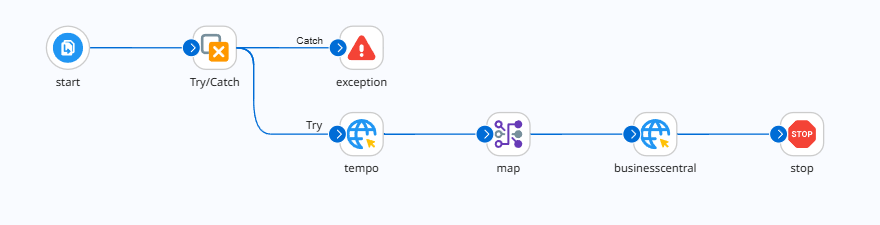
\includegraphics[width=\textwidth,height=\textheight,keepaspectratio]{../bachproef/images/Boomi_AtlassianTime.png}
    \caption{Boomi: data integratie tussen Atlassian Tempo en Microsoft Business Central}
\end{figure}

\begin{figure}[H]
    \centering
    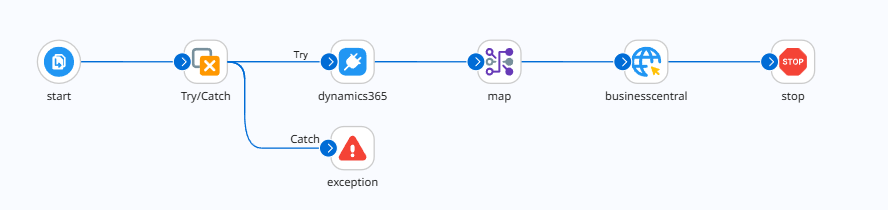
\includegraphics[width=\textwidth,height=\textheight,keepaspectratio]{../bachproef/images/Boomi_Quote_Creation.png}
    \caption{Boomi: data integratie tussen Microsoft Dynamics Sales en Microsoft Business Central}
\end{figure}

\begin{figure}[H]
    \centering
    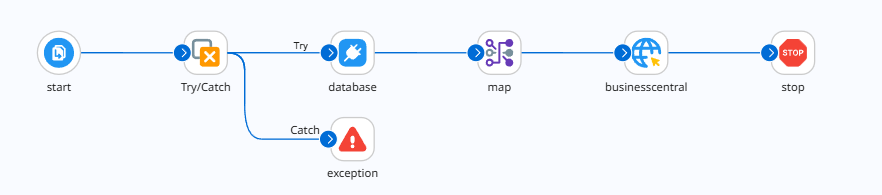
\includegraphics[width=\textwidth,height=\textheight,keepaspectratio]{../bachproef/images/Boomi_Database_BusinessCentral.png}
    \caption{Boomi: data integratie tussen Microsoft SQL Server en Microsoft Business Central}
\end{figure}

\vspace{\baselineskip}

\textbf{Automatisering van processen: Manuele administratieve taken moeten geautomatiseerd kunnen worden om fouten te verminderen en bepaalde processen te versnellen.}

\vspace{\baselineskip}

Boomi beschikt over de mogelijkheid om taken manueel en automatisch uit te voeren. Manuele processen kunnen via de website handmatig uitgevoerd worden. Geplande of tijdgestuurde uitvoeringen kunnen dagelijks, wekelijks, maandelijks of op specifiek geplande dagen automatisch uitgevoerd worden. Tenslotte is het ook mogelijk om processen reactief uit te voeren als een soort event-driven proces aan de hand van webhooks, database triggers of andere events.

Voor dit requirement scoort Boomi een 4.


\vspace{\baselineskip}
\textbf{Data-transformatie: Het platform moet data makkelijk kunnen converteren tussen verschillende formaten en structuren (bijv. XML ↔ JSON, CSV ↔ database records).}

\vspace{\baselineskip}

Boomi beschikt over een mapping component dat het mogelijk maakt om data van verschillende datatypen te converteren naar het gewenste data type. In de mapping component kan er gekozen worden uit de volgende datatypen om te converteren:

\begin{itemize}
    \item XML
    \item JSON
    \item Flat file
    \item EDI
    \item Database (legacy)
\end{itemize}

Voor dit requirement scoort Boomi een 5.


\vspace{\baselineskip}


\textbf{Monitoring en logging: Het systeem moet real-time monitoring en logboek functionaliteiten bieden om fouten en prestaties bij te houden.}

\vspace{\baselineskip}

Boomi biedt de mogelijkheid aan om data integraties te monitoren, controleren en te testen. Met ook de mogelijkheid om fouten op te vangen. Voor monitoring maakt Boomi gebruik van een ingebouwde Process Reporting Console waarmee gebruikers in real-time informatie krijgen over de status van integratieprocessen. Het dashboard toont informatie over huidige en historische data integraties inclusief fouten, waarschuwingen en doorlooptijden. Bij het uitvoeren van een data integratie wordt er ook een logboek gecreëerd waarin informatie wordt weergegeven over de tijdsduur van het proces, de verwerkte records, eventuele foutmeldingen en informatie over waar de fout heeft plaatsgevonden. Bij het opstellen van de data integraties zelf is het ook mogelijk om fouten op te vangen aan de hand van een try/catch systeem of andere vormen van logische poorten indien er iets fout gaat gedurende het proces. Het is ook mogelijk via configuraties om alerts te sturen via email of integraties te maken met externe monitoring tools.

Voor dit requirement scoort Boomi een 5.


\vspace{\baselineskip}

\subsection{Should have}%
\label{ShouldHaveBoomi}

\textbf{Kostenbeheersing: De tool moet betaalbaar zijn met een transparant kostenmodel (licenties, onderhoud, implementatie).}

\vspace{\baselineskip}

Van alle drie de integratie tools is Boomi het minst transparant over de exacte kosten van hun software en services. Boomi heeft namelijk 2 kostenmodellen waaruit de klant kan kiezen namelijk:

\vspace{\baselineskip}

Een abonnementsstructuur waarbij de klant kan kiezen uit 4 opties naargelang de wensen en de grootte van het bedrijf hierbij wordt er geen exacte prijs op voorhand aangegeven en moet er onderhandeld worden met het sales team van Boomi voor een abonnement op maakt uit te werken. Hieronder worden de 4 abonnement modellen kort toegelicht voor een idee te geven van hun schaal:

\begin{itemize}
    \item Base Edition: geschikt voor eenvoudige integraties.
    \item Professional Edition: voor meerdere applicaties en basis-API-ondersteuning.
    \item Enterprise Edition:  gericht op complexe integraties, API management, en EDI.
    \item Enterprise Plus / Ultimate:  voor organisaties met zeer hoge schaal- en governance-eisen.
\end{itemize}

Als tweede betaaloptie biedt Boomi ook nog een pay-as-you-go model aan waarbij de klant maandelijks 99 dollar moet betalen als basisprijs + extra verbruikskosten afhankelijk van het verbruik dat het bedrijf maandelijks maakt. De exacte bedragen voor deze verbruikskosten worden helaas niet op de website weergegeven en ook hiervoor zal er contact opgenomen moeten worden met het sales team van Boomi.

Tenslotte is er ook de mogelijkheid om Boomi gratis voor 30 dagen uit te proberen om een inkijk te geven in het ecosysteem van Boomi. Na 30 dagen wordt het trial-account wel verwijderd dus hiervoor moet opgelet worden indien er na een testfase zou gekozen worden om Boomi verder te gebruiken.

Voor dit requirement scoort Boomi een 3.

\vspace{\baselineskip}

\textbf{Schaalbaarheid: De tool moet eenvoudig schaalbaar zijn naargelang de wensen van de organisatie.}

\vspace{\baselineskip}

Boomi kan hun systemen perfect schalen naargelang de wensen van de klant. Deze schaalbaarheid is wel afhankelijk van het vooraf afgesproken contract dat het bedrijf heeft met Boomi. Het is perfect mogelijk om de schaalbaarheid te wijzigen indien nodig, maar hiervoor kan het zijn dat bedrijven contact moeten opnemen met Boomi om hun contract te wijzigen naargelang de grootte van de schaal die gewijzigd moet worden.

Voor dit requirement scoort Boomi een 4.


\vspace{\baselineskip}

\textbf{Connectoren en adapters: Het platform moet kant-en-klare connectoren bieden voor veelgebruikte systemen (bijv. SAP, Microsoft Dynamics, Oracle).}
\vspace{\baselineskip}

Boomi beschikt over een enorm aanbod aan kant-en-klare connectoren om connecties te maken met welgekende systemen zoals SAP, Amazon, Microsoft Dynamics, Oracle, Salesforce, Azure en andere grote bedrijven. Toch beschikt Boomi niet over alle connectoren die Axians zou nodig hebben. Zo is er voor Atlassian Tempo in geen enkele vorm een beschikbare kant-en-klare connector beschikbaar en moest deze zelf aangemaakt worden. Voor andere niche systemen zal er waarschijnlijk ook gezien moeten worden om eigen custom connectoren aan te maken.  

Voor dit requirement scoort Boomi een 4.


\vspace{\baselineskip}

\textbf{Prestaties: De tool moet performant zijn bij het uitvoeren van bepaalde veelgebruikte data integraties, maar niet alle data integratie processen.}

\vspace{\baselineskip}

Boomi presteert goed bij standaard en veelvoorkomende data integraties, vooral in cloudomgevingen. Bij minder traditionele, complexere of data intensieve processen kan de performance licht tegenvallen door beperkingen in optimalisatie. Gezien de requirement stelt dat niet alle processen performant moeten zijn, scoort Boomi relatief goed, zolang de focus op de standaardintegraties ligt zoals de data integratie tussen Microsoft Dynamics Sales en Microsoft Business Central.

Voor dit requirement scoort Boomi een 4.

\vspace{\baselineskip}

\textbf{Onderhoudsvriendelijkheid: De tool moet eenvoudig te updaten en te onderhouden zijn met minimale downtime.}

\vspace{\baselineskip}

Boomi biedt een service level agreement van 99.99 \% uptime aan en houdt ook een revisie geschiedenis aan dat aantoont welke aanpassingen er zijn gemaakt door wie en ook wanneer deze wijzigingen plaatsvonden. Eerdere versies van een data integratie kunnen aangevraagd worden en ook opnieuw bewerkt worden. Upates worden ook automatisch uitgevoerd.

Voor dit requirement scoort Boomi een 4.

\vspace{\baselineskip}

\subsection{Could have}%
\label{CouldHaveBoomi}

\textbf{Hybrid en multi-cloud ondersteuning: Het platform moet applicaties kunnen integreren die draaien in verschillende omgevingen (on-premise, private cloud, public cloud).}

\vspace{\baselineskip}

Boomi biedt een uitgebreide ondersteuning voor on-premise, hybrid en multi-cloud integraties, met sterke tools voor connectiviteit, deployment en beheer. Het platform is gebruiksvriendelijk, maar kan in zeer complexe of sterk beveiligde omgevingen nog enige aanpassing of extra tooling vereisen.

Voor dit requirement scoort Boomi een 4.

\vspace{\baselineskip}

\textbf{Low-code / no-code interface: Het platform beschikt over een low-code of no-code interface voor het aanmaken van data integraties.}

\vspace{\baselineskip}

Boomi biedt sterke low-code capaciteiten en een gebruiksvriendelijk interface die veel integraties mogelijk maakt zonder diepgaande technische kennis. Langs de no-code kant lijkt het requirement niet volledig haalbaar bij complexere scenario's en voor meer geadvanceerde data integraties is technische expertise tamelijk nodig.

Voor dit requirement scoort Boomi een 4.

\newpage

\begin{landscape}

\subsection{Eindoverzicht}%
\label{EindoverzichtBoomi}

\begin{table}[H]
\centering
\resizebox{\linewidth}{!}{% resize the table to fit page width
\begin{tabular}{|ll|}
\hline
\multicolumn{1}{|l|}{\textbf{Requirements uit de requirementsanalyse}}                                                                                                                                                     & \textbf{Score tussen 1 en 5} \\ \hline
\textbf{Must have}                                                                                                                                                                                                         &                              \\ \hline
\multicolumn{1}{|l|}{Veiligheid en betrouwbaarheid: De tool moet voldoen aan de relevante beveiligingsnormen (Welbekende ISO-normen, data-encryptie, Europese GDPR-wetgeving compliance).}                                 & 4                            \\ \hline
\multicolumn{1}{|l|}{Uitbreidbaarheid: De tool moet eenvoudig uitbreidbaar zijn met nieuwe modules en integraties naarmate de organisatie groeit.}                                                                         & 4                            \\ \hline
\multicolumn{1}{|l|}{Integratie van meerdere systemen: Het platform moet in staat zijn om verschillende applicaties en systemen met elkaar te verbinden (zoals ERP, CRM, HRM, legacy-systemen, databases) met elkaar te verbinden.} & 4                            \\ \hline
\multicolumn{1}{|l|}{Automatisering van processen: Manuele administratieve taken moeten geautomatiseerd kunnen worden om fouten te verminderen en bepaalde processen te versnellen.}                                       & 4                            \\ \hline
\multicolumn{1}{|l|}{Data-transformatie: Het platform moet data makkelijk kunnen converteren tussen verschillende formaten en structuren (bijv. XML ↔ JSON, CSV ↔ database records).}                                      & 5                            \\ \hline
\multicolumn{1}{|l|}{Monitoring en logging: Het systeem moet real-time monitoring en logboek functionaliteiten bieden om fouten en prestaties bij te houden.}                                                              & 5                            \\ \hline
\textbf{Should have}                                                                                                                                                                                                       &                              \\ \hline
\multicolumn{1}{|l|}{Kostenbeheersing: De tool moet betaalbaar zijn met een transparant kostenmodel (licenties, onderhoud, implementatie).}                                                                                & 3                            \\ \hline
\multicolumn{1}{|l|}{Schaalbaarheid: De tool moet eenvoudig schaalbaar zijn naargelang de wensen van de organisatie.}                                                                                                      & 4                            \\ \hline
\multicolumn{1}{|l|}{Connectoren en adapters: Het platform moet kant-en-klare connectoren bieden voor veelgebruikte systemen (bijv. SAP, Microsoft Dynamics, Oracle).}                                                     & 4                            \\ \hline
\multicolumn{1}{|l|}{Prestaties: De tool moet performant zijn bij het uitvoeren van bepaalde veelgebruikte data integraties, maar niet alle data integratie processen.}                                                    & 4                            \\ \hline
\multicolumn{1}{|l|}{Onderhoudsvriendelijkheid: De tool moet eenvoudig te updaten en te onderhouden zijn met minimale downtime.}                                                                                           & 4                            \\ \hline
\textbf{Could have}                                                                                                                                                                                                        &                              \\ \hline
\multicolumn{1}{|l|}{Hybrid en multi-cloud ondersteuning: Het platform moet applicaties kunnen integreren die draaien in verschillende omgevingen (on-premise, private cloud, public cloud).}                              & 4                            \\ \hline
\multicolumn{1}{|l|}{Low-code / no-code interface: Het platform beschikt over een low-code of no-code interface voor het aanmaken van data integraties.}                                                                   & 4                            \\ \hline
\multicolumn{1}{|l|}{\textbf{Gemiddelde}}                                                                                                                                                                                  & 4,08                         \\ \hline
\multicolumn{1}{|l|}{\textbf{Mediaan}}                                                                                                                                                                                     & 4                            \\ \hline
\end{tabular}
}
\caption{Boomi: Beoordeling van requirements op een schaal van 1 tot 5}
\end{table}

\end{landscape}
\chapter{\IfLanguageName{dutch}{Zapier}{Zapier}}
\label{ch:Zapier}

De tweede integratie tool waarvan de resultaten zullen besproken worden is Zapier. Hieronder worden de requirements individueel besproken en krijgen ze een score tussen 1 (voldoet niet aan de verwachtingen) en 5 (voldoet aan alle verwachtingen) toegewezen. Op het einde van het hoofdstuk worden alle requirements en hun scores samengevat en weergegeven in een tabel met enkele extra berekeningen om het vergelijkingsproces te vereenvoudigen.

\section{Requirements}%
\label{RequirementsZapier}

\subsection{Must have}%
\label{MustHaveZapier}

\textbf{Veiligheid en betrouwbaarheid: De tool moet voldoen aan de relevante beveiligingsnormen (Welbekende ISO-normen, data-encryptie, Europese GDPR-wetgeving compliance).}

\vspace{\baselineskip}

Op vlak van veiligheid en betrouwbaarheid beschikt Zapier niet over dezelfde zekerheden zoals de andere data integratie platformen. Zo beschikt Zapier over geen enkel ISO-certificaat. Het beschikt wel over een Trust Center en communiceert duidelijk over beveiligingsmaatregelen, waaronder penetratietests en beveiligings audits. Waar Zapier wel over beschikt op vlak van certificaten is een SOC2 Type II en een SOC 3 certificaat voor onafhankelijke controles van interne processen en gegevensbescherming. Op vlak van data-encryptie maakt Zapier gebruik van TLS 1.2/1.3 voor encryptie tijdens transport en AES-256 tijdens rust. Zapier voldoet ook aan de Europese GDPR-wetgeving, maar blijven er wel risico’s doordat er een data overdracht is naar de VS en de klant beperkte controle heeft over de opslagplaats van gegevens. Er kunnen dus veiligheidsproblemen zijn met zeer gevoelige gegevens. Op vlak van authenticatie en autorisatie ondersteunt Zapier OAuth 2.0 en zijn er voor zakelijke gebruikers mogelijkheden tot rolgebaseerde toegangscontrole (RBAC), audit logs en teambeheer via de Zapier for Teams/Companies abonnementsformules. 


Voor dit requirement scoort Zapier een 2.

\vspace{\baselineskip}

\textbf{Uitbreidbaarheid: De tool moet eenvoudig uitbreidbaar zijn met nieuwe modules en integraties naarmate de organisatie groeit.}

\vspace{\baselineskip}

Zapier is goed uitbreidbaar op vlak van het toevoegen van nieuwe data integraties en nieuwe modules. Zo kan er op het platform een onbeperkt aantal aan nieuwe data integraties worden toegevoegd, maar moet de gebruiker opletten dat de gekozen of afgesproken abonnementsstructuur over voldoende tasks beschikt om deze nieuwe data integraties te ondersteunen. Tasks in deze context zijn alle acties die een data integratie uitvoeren na de activatie van de trigger. De hoeveelheid tasks die uitgevoerd kunnen worden hangt af van de geselecteerde hoeveelheid bij de start van het abonnement of wat onderling afgesproken is voor de Enterprise edition. Zapier biedt ook de mogelijkheid voor nieuwe connectoren aan te maken via webhooks of “Code by Zapier” voor integraties buiten het ecosysteem. Helaas is er weinig tot geen native ondersteuning voor het ontwikkelen van herbruikbare modules, subflows of templates die complexere logica blokken efficiënt kunnen hergebruiken. Daardoor kan onderhoud lastig worden naarmate de hoeveelheid data integraties stijgt.


Voor dit requirement scoort Zapier een 3.

\vspace{\baselineskip}

\textbf{Integratie van meerdere systemen: Het platform moet in staat zijn om verschillende applicaties en systemen met elkaar te verbinden (zoals ERP, CRM, HRM, legacy-systemen, databases) met elkaar te verbinden.}

\vspace{\baselineskip}

Zapier is sterk in het koppelen van simpele en cloudgebaseerde applicaties, maar biedt weinig tot geen ondersteuning voor data integraties met on-premise, legacy of gespecialiseerde ERP, HRM of CRM-oplossingen tenzij deze systemen of applicaties beschikken over een API-laag of een connector van een derde partij die wel kan koppelen met deze systemen of applicaties. Het platform mist hierdoor functionaliteit en compatibiliteit met traditionele on-premise, ERP- en legacy-omgevingen doordat het platform ontworpen is met het cloud-first principe. Tenslotte kunnen er ook problemen ontstaan wanneer bepaalde data-integraties complexer of uitgebreid worden. Hiermee kan enkel geconcludeerd worden dat Zapier over onvoldoende middelen en functionaliteiten beschikt om aan de eisen van enterprise data integration te voldoen.

\vspace{\baselineskip}

Door een probleem met bepaalde connectoren en conversies is de proof of concept voor dit data integration platform mislukt en kunnen enkel hypothetische data integraties getoond worden. Deze hypothetische integraties zijn in de bijlage geplaatst door de grootte van de figuren. Zie bijlage: \ref{ch:Zapier1}, \ref{ch:Zapier2} en \ref{ch:Zapier3}

Voor dit requirement scoort Zapier een 2.


\vspace{\baselineskip}

\textbf{Automatisering van processen: Manuele administratieve taken moeten geautomatiseerd kunnen worden om fouten te verminderen en bepaalde processen te versnellen.}

\vspace{\baselineskip}

Zapier beschikt over de mogelijkheid om taken manueel, automatisch of aan de hand van events of triggers uit te voeren. Het platform focust zich hoofdzakelijk op event-driven automatisatie waarbij data integraties geactiveerd worden op basis van een vooraf bepaald event zoals het toevoegen van een nieuwe rij data in een dataset. Helaas is de flexibiliteit van de event-driven of automatische integraties veel beperkter dan de andere 2 data integratie platformen. Zo ondersteunt Zapier geen geavanceerde tijdgebaseerde planningen en is er een gebrek aan ondersteuning voor het instellen van complexe workflow-modellering.


Voor dit requirement scoort Zapier een 3.

\vspace{\baselineskip}
\textbf{Data-transformatie: Het platform moet data makkelijk kunnen converteren tussen verschillende formaten en structuren (bijv. XML ↔ JSON, CSV ↔ database records).}

\vspace{\baselineskip}

Zapier beschikt over een zeer gelimiteerd arsenaal aan data-transformatie mogelijkheden. Zo beschikt het platform wel over data-transformatie op vlak van tekst splitsing of samenvoeging, datum-/tijd conversies, het zoeken en vervangen van data, het uitvoeren van numerieke berekeningen, het opschonen van teksten, het formatteren van valuta, telefoonnummers en getallen, maar is er geen ingebouwde ondersteuning voor het transformeren of mappen van XML, JSON, CSV of database records. Indien een gebruiker toch wenst aan data-transformatie te doen, is dit enkel mogelijk door gebruik te maken van de “Code by Zapier” module waarbij de gebruiker zelf een script moet schrijven in Python of JavaScript voor de conversie van de data.

Voor dit requirement scoort Zapier een 1.


\vspace{\baselineskip}


\textbf{Monitoring en logging: Het systeem moet real-time monitoring en logboek functionaliteiten bieden om fouten en prestaties bij te houden.}

\vspace{\baselineskip}

Zapier beschikt over een basisvorm van real-time monitoring en logging tijdens de uitvoering van data integraties. Zo beschikt Zapier over een status dashboard waarbij een logboek wordt bijgehouden van alle data integraties met hun trigger gegevens, actie gegevens, eventuele foutmeldingen en de duurtijd van iedere stap in de data integratie. De gebruiker kan optioneel ook direct op de hoogte worden gebracht via mail of app-notificatie van zodra een data integratie faalt. Desondanks blijft de monitoring van Zapier beperkt wanneer een gebruiker diepgaande analyses of vergelijkingen wil doen van de data integraties. Zo is het moeilijk om trends in prestaties of foutmeldingen te analyseren.


Voor dit requirement scoort Zapier een 3.


\vspace{\baselineskip}

\subsection{Should have}%
\label{ShouldHaveZapier}

\textbf{Kostenbeheersing: De tool moet betaalbaar zijn met een transparant kostenmodel (licenties, onderhoud, implementatie).}

\vspace{\baselineskip}

Op vlak van prijstransparantie scoort Zapier vrij goed. Het maakt gebruik van een abonnementsstructuur waarbij bijna alle betalende opties een vaste zichtbare prijs tonen. De klant kan ook kiezen om zich op maandelijkse en jaarlijkse intervals te abonneren voor de service met als voordeel dat de klant 33 \% korting krijgt op de totaalprijs indien gekozen wordt voor de jaarlijkse formule. Dit geeft de klant enorm veel flexibiliteit in hoe hij de service wil gebruiken. De prijs kan wel beïnvloed worden door de hoeveelheid tasks die de klant maandelijks wenst uit te voeren, maar dit kan op voorhand geselecteerd worden om zo de exacte prijs weer te geven.

\vspace{\baselineskip}

De abonnementsstructuur bestaat uit 3 opties waaruit de klant kan kiezen, elk aangepast naar de mate van specifieke doelgroepen. Hierbij werd uitgegaan van een verbruik van 2000 tasks per maand en aangerekend op maandelijkse basis (zonder de jaarkorting van 33 \%). Hieronder worden de 3 abonnement modellen kort toegelicht voor een idee te geven van hun schaal en wat ze exact aanbieden:

\begin{itemize}
    \item Professional: € 66,47 per maand gericht naar individuele gebruikers.
    \item Team: € 93,60 per maand gericht naar bedrijven van teams tot en met 25 gebruikers.
    \item Enterprise: Geen concrete prijs. Abonnement volledig afgestemd op de wensen van het bedrijf. Gericht naar zeer grote bedrijven met verschillende departementen die gebruik willen maken van de integratie tool.
\end{itemize}

Tenslotte is er ook de mogelijkheid om Zapier gratis voor 14 dagen uit te proberen om een inkijk te geven in het ecosysteem van Zapier. Na deze periode wordt het trial account behouden, maar worden alle Flows met premium features stopgezet en wordt het account omgezet naar een gratis versie.

Voor dit requirement scoort Zapier een 4.

\vspace{\baselineskip}

\textbf{Schaalbaarheid: De tool moet eenvoudig schaalbaar zijn naargelang de wensen van de organisatie.}

\vspace{\baselineskip}

Zapier is relatief beperkt op vlak van schaalbaarheid. Veel van de schaalbaarheid van Zapier is afhankelijk van de gekozen of afgesproken abonnementsstructuur en de daaraan gekoppelde hoeveelheid uitvoerbare tasks per maand. Hierdoor schaalt Zapier goed voor kleine tot middelgrote ondernemingen, maar kan het relatief beperkt aanvoelen voor complexe enterprise data integraties, integraties met een zware workload of integraties die intensief gebruikt worden. Met de enterprise abonnement optie beschikt een gebruiker wel over een bepaalde vorm van schaalbaarheid die kan bepaald worden. Bij de andere standaard abonnementsvormen kan enkel de hoeveelheid tasks per maand flexibel gekozen worden.


Voor dit requirement scoort Zapier een 3.


\vspace{\baselineskip}

\textbf{Connectoren en adapters: Het platform moet kant-en-klare connectoren bieden voor veelgebruikte systemen (bijv. SAP, Microsoft Dynamics, Oracle).}
\vspace{\baselineskip}

Zapier is uitstekend in het integreren van moderne, simpele en veelgebruikte cloud applicaties zoals Google Workspace, Slack en non-enterprise Microsoft software, maar stelt teleur als het gaat om kant-en-klare connectoren voor enterprise-systemen zoals SAP, Oracle en de Microsoft Dynamics software op vlak van ondersteuning. Indien Zapier niet beschikt over een directe connector biedt Zapier wel de optie om via Webhooks of de “Code by Zapier”-module zelf connectoren aan te maken, maar voelde veel beperkter aan dan de andere data integratie softwares. Wat ook zeer merkbaar is, is dat Zapier zeer afhankelijk is van publieke api’s en weinig tot geen ondersteuning biedt voor legacy of on-premise systemen.


Voor dit requirement scoort Zapier een 2.


\vspace{\baselineskip}

\textbf{Prestaties: De tool moet performant zijn bij het uitvoeren van bepaalde veelgebruikte data integraties, maar niet alle data integratie processen.}

\vspace{\baselineskip}

Zapier levert degelijke prestaties voor standaard, lichte data integraties tussen veelgebruikte apps. Helaas bij het uitvoeren van complexe, data-intensieve of realtime data integraties kan de performance vrij beperkt of gebrekkig aanvoelen. Zo kan de polling (het periodiek controleren van data of er iets gewijzigd is) soms tot 15 minuten vertraging oplopen bij de gratis of instapversie van Zapier. Deze latency kan wel drastisch verlaagt worden tot 1 minuut door over te schakelen naar een hoger abonnementniveau. Ook moet er rekening gehouden worden met de limieten op vlak van aantal taken per maand dat uitgevoerd kan worden, afhankelijk van het abonnement. Dit kan soms leiden tot een vertraagde uitvoering van taken. Tenslotte is er ook een maximale looptijd per taak van 30 seconden, wat een probleem kan vormen bij zware data-intensieve processen zoals het ophalen van bulk-data uit een database. 


Voor dit requirement scoort Zapier een 3.


\vspace{\baselineskip}

\textbf{Onderhoudsvriendelijkheid: De tool moet eenvoudig te updaten en te onderhouden zijn met minimale downtime.}

\vspace{\baselineskip}

Zapier biedt een service level agreement van 99.99 \% uptime aan en draait volledig in de cloud als een SaaS-oplossing (Software as a Service). Wat er ook voor zorgt dat updates automatisch worden uitgevoerd. Helaas beperkt Zapier over zeer beperkte versie controle of rollback-mogelijkheden. Het is daardoor lastig om grote wijzigingen te beheren of terug te keren naar een eerdere staat indien er iets fout is gegaan. Ook beschikt Zapier niet over een changelog die weergeeft welke veranderingen er zijn gebeurd tussen verschillende versies. 


Voor dit requirement scoort Zapier een 3.


\vspace{\baselineskip}

\subsection{Could have}%
\label{CouldHaveZapier}

\textbf{Hybrid en multi-cloud ondersteuning: Het platform moet applicaties kunnen integreren die draaien in verschillende omgevingen (on-premise, private cloud, public cloud).}

\vspace{\baselineskip}

Zapier is het best geschikt voor integraties binnen de publieke cloud, maar faalt grotendeels als het gaat om hybride of private cloud omgevingen. Door een gebrek aan native ondersteuning voor on-premise of private cloud integraties maakt het platform zichzelf zeer onbruikbaar voor data-integraties die plaatsvinden buiten de public cloud. Indien de gebruiker toch wenst gebruik te maken van systemen buiten de public cloud zullen er tussenoplossingen voorzien moeten worden zoals een custom API-server of webhook, wat op zijn beurt mogelijke veiligheidsproblemen kan meebrengen.


Voor dit requirement scoort Zapier een 2.


\vspace{\baselineskip}

\textbf{Low-code / no-code interface: Het platform beschikt over een low-code of no-code interface voor het aanmaken van data integraties.}

\vspace{\baselineskip}

Zapier biedt een ruim aanbod aan low-code en no-code mogelijkheden voor het aanmaken van data integraties met een zeer gebruiksvriendelijke interface. Diepe of sterke technische kennis is niet noodzakelijk voor het aanmaken van simpele of standaard data integraties. Bij meer complexe data integraties kan deze simplistische interface wel beperkingen of gebreken oplopen, wat ervoor kan zorgen dat de gebruiker sommige aspecten in het integratieproces manueel moet coderen.

Voor dit requirement scoort Zapier een 3.


\newpage

\begin{landscape}



\subsection{Eindoverzicht}%
\label{EindoverzichtZapier}

\begin{table}[H]
\centering
\resizebox{\linewidth}{!}{% resize the table to fit page width
\begin{tabular}{|ll|}
\hline
\multicolumn{1}{|l|}{\textbf{Requirements uit de requirementsanalyse}}                                                                                                                                                     & \textbf{Score tussen 1 en 5} \\ \hline
\textbf{Must have}                                                                                                                                                                                                         &                              \\ \hline
\multicolumn{1}{|l|}{Veiligheid en betrouwbaarheid: De tool moet voldoen aan de relevante beveiligingsnormen (Welbekende ISO-normen, data-encryptie, Europese GDPR-wetgeving compliance).}                                 & 2                            \\ \hline
\multicolumn{1}{|l|}{Uitbreidbaarheid: De tool moet eenvoudig uitbreidbaar zijn met nieuwe modules en integraties naarmate de organisatie groeit.}                                                                         & 3                            \\ \hline
\multicolumn{1}{|l|}{Integratie van meerdere systemen: Het platform moet in staat zijn om verschillende applicaties en systemen met elkaar te verbinden (zoals ERP, CRM, HRM, legacy-systemen, databases) met elkaar te verbinden.} & 2                            \\ \hline
\multicolumn{1}{|l|}{Automatisering van processen: Manuele administratieve taken moeten geautomatiseerd kunnen worden om fouten te verminderen en bepaalde processen te versnellen.}                                       & 3                            \\ \hline
\multicolumn{1}{|l|}{Data-transformatie: Het platform moet data makkelijk kunnen converteren tussen verschillende formaten en structuren (bijv. XML ↔ JSON, CSV ↔ database records).}                                      & 1                            \\ \hline
\multicolumn{1}{|l|}{Monitoring en logging: Het systeem moet real-time monitoring en logboek functionaliteiten bieden om fouten en prestaties bij te houden.}                                                              & 3                            \\ \hline
\textbf{Should have}                                                                                                                                                                                                       &                              \\ \hline
\multicolumn{1}{|l|}{Kostenbeheersing: De tool moet betaalbaar zijn met een transparant kostenmodel (licenties, onderhoud, implementatie).}                                                                                & 4                            \\ \hline
\multicolumn{1}{|l|}{Schaalbaarheid: De tool moet eenvoudig schaalbaar zijn naargelang de wensen van de organisatie.}                                                                                                      & 3                            \\ \hline
\multicolumn{1}{|l|}{Connectoren en adapters: Het platform moet kant-en-klare connectoren bieden voor veelgebruikte systemen (bijv. SAP, Microsoft Dynamics, Oracle).}                                                     & 2                            \\ \hline
\multicolumn{1}{|l|}{Prestaties: De tool moet performant zijn bij het uitvoeren van bepaalde veelgebruikte data integraties, maar niet alle data integratie processen.}                                                    & 3                            \\ \hline
\multicolumn{1}{|l|}{Onderhoudsvriendelijkheid: De tool moet eenvoudig te updaten en te onderhouden zijn met minimale downtime.}                                                                                           & 3                            \\ \hline
\textbf{Could have}                                                                                                                                                                                                        &                              \\ \hline
\multicolumn{1}{|l|}{Hybrid en multi-cloud ondersteuning: Het platform moet applicaties kunnen integreren die draaien in verschillende omgevingen (on-premise, private cloud, public cloud).}                              & 2                            \\ \hline
\multicolumn{1}{|l|}{Low-code / no-code interface: Het platform beschikt over een low-code of no-code interface voor het aanmaken van data integraties.}                                                                   & 3                            \\ \hline
\multicolumn{1}{|l|}{\textbf{Gemiddelde}}                                                                                                                                                                                  & 2,62                            \\ \hline
\multicolumn{1}{|l|}{\textbf{Mediaan}}                                                                                                                                                                                     & 3                            \\ \hline
\end{tabular}
}
\caption{Zapier: Beoordeling van requirements op een schaal van 1 tot 5}
\end{table}

\end{landscape}
\chapter{\IfLanguageName{dutch}{Microsoft Power Automate}{Microsoft Power Automate}}
\label{ch:Microsoft}

De laatste integratie tool waarvan de resultaten zullen besproken worden is Microsoft Power Automate. Hieronder worden de requirements individueel besproken en krijgen ze een score tussen 1 (voldoet niet aan de verwachtingen) en 5 (voldoet aan alle verwachtingen) toegewezen. Op het einde van het hoofdstuk worden alle requirements en hun scores samengevat en weergegeven in een tabel met enkele extra berekeningen om het vergelijkingsproces te vereenvoudigen.

\section{Requirements}%
\label{RequirementsMicrosoft}

Om deze review iets vlotter leesbaar te maken zal Microsoft Power Automate afgekort worden tot Microsoft of MicrosoftPA gedurende deze review.

\subsection{Must have}%
\label{MustHaveMicrosoft}

\textbf{Veiligheid en betrouwbaarheid: De tool moet voldoen aan de relevante beveiligingsnormen (Welbekende ISO-normen, data-encryptie, Europese GDPR-wetgeving compliance).}

\vspace{\baselineskip}

Microsoft is wereldwijd bekend om hun veilige en betrouwbare producten en diensten. Hun data integratie tool Microsoft Power Automate draait in de cloud op het Microsoft Azure-platform. Hierdoor beschikt het data integratie platform over verschillende ISO-normen, sterke en flexibele data-encryptie en voldoet het platform ook aan de eisen van de Europese GDPR-wetgeving. Op vlak van ISO-normen beschikt MicrosoftPI over ISO/IEC 27001 voor informatiebeveiliging management, ISO/IEC 27018 voor de bescherming van persoonlijke gegevens in de cloud en ISO/IEC 27701 voor Privacy Information Management. Op vlak van data-encryptie gebruikt MicrosoftPA "in transit" (TLS 1.2+) en "at rest" (Azure Storage Service Encryption) om data te beveiligen. Microsoft biedt ook de mogelijkheid om zelf versleuteling in te stellen met persoonlijke encryptiesleutels (Customer Managed Keys). Voor autorisatie maakt Microsoft ook gebruik van Role-based access control (RBAC) voor een overzichtelijke en veilige toegangscontrole.


Voor dit requirement scoort Microsoft een 5.

\vspace{\baselineskip}

\textbf{Uitbreidbaarheid: De tool moet eenvoudig uitbreidbaar zijn met nieuwe modules en integraties naarmate de organisatie groeit.}

\vspace{\baselineskip}

MicrosoftPA beschikt over een ruim aanbod aan mogelijkheden op vlak van uitbreidingen. Zo kan het platform gebruik maken van verschillende Microsoft enterprise-tools om de kwaliteit en functionaliteit van de service te verbeteren. Voor deze services zijn vaak wel meerdere of hogere licenties nodig. MicrosoftPA geeft wel de mogelijkheid om eigen custom connectoren aan te maken. Hiermee kunnen de beschikbare data integraties kunnen worden uitgebreid voor bepaalde maatwerk data-integraties. In hoeverre de standaard licenties voor MicrosoftPA uitbreidbaarheid toelaten is onzeker. De limiet voor uitbreidbaarheid lijkt gekoppeld te zijn aan het plafond van de gekozen licentie, wat beperkingen kan opleggen op vlak van flexibiliteit. 


Voor dit requirement scoort Microsoft een 4.


\vspace{\baselineskip}

\textbf{Integratie van meerdere systemen: Het platform moet in staat zijn om verschillende applicaties en systemen met elkaar te verbinden (zoals ERP, CRM, HRM, legacy-systemen, databases) met elkaar te verbinden.}

\vspace{\baselineskip}

MicrosoftPA is in staat om verschillende applicaties en systemen met elkaar te kunnen verbinden aan de hand van data integraties. Voor 2 van de 3 data integraties is het zelf mogelijk om de data integraties te bouwen met enkel de ingebouwde componenten van Microsoft doordat de integratie plaatsvond tussen 2 microsoft services. Voor de andere data integratie moest gebruikgemaakt worden van een http component om verbinding te kunnen maken met Atlassian Tempo. Hiermee is Microsoft uitstekend voor alle data integraties die plaatsvinden tussen verschillende Microsoft systemen en kan het ook goed omgaan met systemen buiten het Microsoft ecosysteem. Het zou dan ook mogelijk moeten zijn om bijna iedere soort data-integratie te kunnen creëren.

\vspace{\baselineskip}

Bij de proof of concept van deze data integratie tool waren er wel enkele problemen naar boven gekomen. Door de beperking van de gebruikte licentie was het niet mogelijk om de data integratie uit te voeren en konden enkel hypothetische data integratie worden opgesteld doordat alle enterprise-level connectoren enkel uitvoerbaar zijn met premium licenties. De aanvraag voor een premium trial werd helaas ook geweigerd. Zie \ref{ch:licentie} voor meer informatie over de gebruikte licentie en zie bijlage: \ref{ch:Microsoft1}, \ref{ch:Microsoft2} en \ref{ch:Microsoft3} voor de hypothetische data integraties.

Voor dit requirement scoort Microsoft een 4.

\vspace{\baselineskip}

\textbf{Automatisering van processen: Manuele administratieve taken moeten geautomatiseerd kunnen worden om fouten te verminderen en bepaalde processen te versnellen.}

\vspace{\baselineskip}

MicrosoftPA beschikt over verschillende manieren voor de uitvoering van data integraties. Het beschikt over een Automated cloud flow voor de automatische uitvoering van data integraties aan de hand van een vooraf bepaalde trigger, een Instant cloud flow voor het manueel triggeren van een data integratie of een scheduled cloud flow waarbij de gebruiker zelf bepaalt wanneer en hoe een data integratie wordt uitgevoerd. Tenslotte beschikt het ook nog over een desktop flow voor het automatiseren van data integraties op de desktop omgeving in plaats van in de cloud. MicrosoftPA biedt ook een tool aan dat deze processen kan evalueren en optimaliseren indien de gebruiker dit wenst.


Voor dit requirement scoort Microsoft een 4.

\vspace{\baselineskip}
\textbf{Data-transformatie: Het platform moet data makkelijk kunnen converteren tussen verschillende formaten en structuren (bijv. XML ↔ JSON, CSV ↔ database records).}

\vspace{\baselineskip}

MicrosoftPA biedt een basisfunctionaliteit aan voor data-transformatie die goed is voor eenvoudige of simpele scenario’s met een lage complexiteit. Bij grootschalige of complexe data-transformaties kunnen er soms tekortkomingen zijn door een gebrek aan een dedicated conversie tool. Ook bij geneste data kunnen er complicaties tevoorschijn komen. Tenslotte biedt MicrosoftPA een slechte ondersteuning voor data afkomstig uit een CSV. Het platform beschikt niet over een native actie voor het omzetten van CSV data naar andere dataformaten. Hiervoor zal een eigen custom parsing script geschreven moeten worden.

Voor dit requirement scoort Microsoft een 3.

\vspace{\baselineskip}


\textbf{Monitoring en logging: Het systeem moet real-time monitoring en logboek functionaliteiten bieden om fouten en prestaties bij te houden.}

\vspace{\baselineskip}

MicrosoftPA biedt degelijke monitoring en logging aan bij individuele data integraties voor het evalueren van operationele data integraties en het monitoren van fouten. Er zijn echter wel beperkingen bij het monitoren en loggen van data integraties op grote schaal door een gebrek aan een centrale monitoring en logging omgeving. Voor grote of complexe omgevingen zijn aanvullende tools of integraties nodig om aan globale monitoring en logging te kunnen doen.

Voor dit requirement scoort Microsoft een 3.

\vspace{\baselineskip}

\subsection{Should have}%
\label{ShouldHaveMicrosoft}

\textbf{Kostenbeheersing: De tool moet betaalbaar zijn met een transparant kostenmodel (licenties, onderhoud, implementatie).}

\vspace{\baselineskip}

Op vlak van prijstransparantie scoort MicrosoftPA vrij goed. Het maakt gebruik van een abonnementsstructuur waarbij alle betalende opties een vaste zichtbare prijs tonen. Het jammere bij deze abonnementsstructuur is dat deze abonnementen enkel op jaarbasis te verkrijgen zijn, wat zorgt voor een enorme beperking in flexibiliteit.  De prijzen voor deze service lijken ook langs de hogere kant te liggen als er niet gekozen wordt voor het individuele abonnement. Het positieve hierbij is wel dat er geen verbruikskosten worden gerekend bovenop de basisprijs.

\vspace{\baselineskip}

De abonnementsstructuur bestaat uit 3 opties waaruit de klant kan kiezen, elk aangepast naar de mate van specifieke doelgroepen. Hieronder worden de 3 abonnement modellen kort toegelicht voor een idee te geven van hun schaal en wat ze exact aanbieden:

\begin{itemize}
    \item Power Automate Premium: \$15.00 per gebruiker per maand op jaarbasis. Gericht naar individuele personen.
    \item Power Automate Process: \$150.00 per bot per maand op jaarbasis. Gericht naar bedrijven die hun belangrijke bedrijfsprocessen willen automatiseren.
    \item Power Automate Hosted Process: \$215.00 per bot per maand op jaarbasis. Gericht naar bedrijven die hun belangrijke bedrijfsprocessen willen automatiseren aan de hand van een virtuele machine dat gehost wordt op het Microsoft Azure platform.
\end{itemize}

Tenslotte is er ook de mogelijkheid om MicrosoftPA gratis voor 30 tot 90 dagen uit te proberen om een inkijk te geven in het ecosysteem van MicrosoftPA. Na deze periode wordt het trial-account behouden, maar worden alle flows met premium features stopgezet en wordt het account omgezet naar een gratis versie.

Voor dit requirement scoort Microsoft een 4.

\vspace{\baselineskip}

\textbf{Schaalbaarheid: De tool moet eenvoudig schaalbaar zijn naargelang de wensen van de organisatie.}

\vspace{\baselineskip}

Het is onzeker hoe schaalbaar MicrosoftPA is buiten de vaste licentiemodellen. Volgens de verwoording van Microsoft zelf lijkt de schaalbaarheid vast te hangen aan het standaard licentiemodel en is er geen mogelijkheid om te schalen buiten de vernoemde licentiemodellen. Het is wel mogelijk om een bepaalde vorm van schaalbaarheid toe te passen door MicrosoftPA te gebruiken in samenwerking met andere Microsoft enterprise -tools. Tenslotte kunnen er ook bepaalde beperkingen zijn op bepaalde connectoren in de vorm van request-limieten en doorvoersnelheid. Dit kan mogelijks voor problemen zorgen bij grootschalige bedrijven die op een constante basis gebruikmaken van bepaalde connectoren. Dit alles zorgt voor een zeer beperkte flexibiliteit op vlak van schaalbaarheid indien de licentiemodellen niet ideaal zijn voor de schaal van het bedrijf.


Voor dit requirement scoort Microsoft een 3.

\vspace{\baselineskip}

\textbf{Connectoren en adapters: Het platform moet kant-en-klare connectoren bieden voor veelgebruikte systemen (bijv. SAP, Microsoft Dynamics, Oracle).}
\vspace{\baselineskip}

MicrosoftPA beschikt over een ruim aanbod aan kant-en-klare connectoren om con-
necties te maken met welgekende systemen zoals SAP, Amazon, Microsoft Dyna-
mics, Oracle, Salesforce, Azure en andere grote bedrijven. Desondanks beschikt ook Microsoft niet over een connector om een rechtstreekse verbinding te maken met Atlassian Tempo en zal hiervoor zelf een connector aangemaakt worden. Waar MicrosoftPA vooral in uitblinkt is bij de connectie binnen het eigen Microsoft-ecosysteem hierbij worden talloze connectoren voorzien voor de verschillende Microsoft systemen met elkaar te verbinden. Voor meer niche en minder populaire systemen waar Microsoft geen connector voor heeft, biedt het de mogelijkheid om zelf je eigen custom connectoren aan te maken voor het gebruik bij de data integraties.


Voor dit requirement scoort Microsoft een 4.

\vspace{\baselineskip}

\textbf{Prestaties: De tool moet performant zijn bij het uitvoeren van bepaalde veelgebruikte data integraties, maar niet alle data integratie processen.}

\vspace{\baselineskip}

Power Automate biedt goede prestaties voor veelvoorkomende en lichtgewicht integraties, zeker binnen het Microsoft-ecosysteem. Voor zwaardere of grootschalige data integraties kunnen de prestaties tegenvallen vanwege limieten of haperingen bij het verwerken van deze data. Deze limieten en haperingen kunnen op hun beurt ervoor zorgen dat data integraties vertragen of zelfs voor zorgen dat er fouten ontstaan in het verwerkingsproces.

Voor dit requirement scoort Microsoft een 3.

\vspace{\baselineskip}

\textbf{Onderhoudsvriendelijkheid: De tool moet eenvoudig te updaten en te onderhouden zijn met minimale downtime.}

\vspace{\baselineskip}

Microsoft biedt een service level agreement van 99.99 \% uptime aan, maar beschikt enkel over basisfunctionaliteiten op vlak van revisie geschiedenis en toont het enkel wie de laatste wijzigingen heeft aangebracht voor publicatie, maar beschikt het niet over een diepgaand of gedetailleerde revisiegeschiedenis of wijzigingslogs. Indien een bedrijf deze functionaliteiten toch wenst kan er wel gebruikgemaakt worden van integraties met Power Platform ALM of Microsoft 365 Compliance Center.


Voor dit requirement scoort Microsoft een 3.

\vspace{\baselineskip}

\subsection{Could have}%
\label{CouldHaveMicrosoft}

\textbf{Hybrid en multi-cloud ondersteuning: Het platform moet applicaties kunnen integreren die draaien in verschillende omgevingen (on-premise, private cloud, public cloud).}

\vspace{\baselineskip}

Microsoft Power Automate ondersteunt on-premise, hybride en multi-cloud omgevingen. Voor on-premise integratie biedt Microsoft ondersteuning voor on-premise systemen via de On-premises Data Gateway. Hiermee kunnen workflows data ophalen of verzenden naar interne systemen zoals lokale databases, ERP’s, of fileshares. Voor cloud omgevingen biedt Microsoft uitstekende verbindingen voor alle data-integraties binnen het Microsoft ecosysteem. Voor andere cloud omgevingen biedt MicrosoftPA integratiemogelijkheden met applicaties zolang ze via API’s of connectors verbonden kunnen worden. Helaas zijn deze integraties buiten het Microsoft systeem minder diepgaand en beperkter dan de Microsoft cloud omgevingen. 


Voor dit requirement scoort Microsoft een 4.

\vspace{\baselineskip}

\textbf{Low-code / no-code interface: Het platform beschikt over een low-code of no-code interface voor het aanmaken van data integraties.}

\vspace{\baselineskip}

MicrosoftPA biedt sterke low-code capaciteiten en een gebruiksvriendelijk interface die veel integraties mogelijk maakt zonder diepgaande technische kennis. Langs de no-code kant lijkt het requirement niet volledig haalbaar bij complexere scenario's en voor meer geadvanceerde data integraties is technische expertise tamelijk nodig.

Voor dit requirement scoort Microsoft een 4.

\newpage

\begin{landscape}



\subsection{Eindoverzicht}%
\label{EindoverzichtMicrosoft}

\begin{table}[H]
\centering
\resizebox{\linewidth}{!}{% resize the table to fit page width
\begin{tabular}{|ll|}
\hline
\multicolumn{1}{|l|}{\textbf{Requirements uit de requirementsanalyse}}                                                                                                                                                     & \textbf{Score tussen 1 en 5} \\ \hline
\textbf{Must have}                                                                                                                                                                                                         &                              \\ \hline
\multicolumn{1}{|l|}{Veiligheid en betrouwbaarheid: De tool moet voldoen aan de relevante beveiligingsnormen (Welbekende ISO-normen, data-encryptie, Europese GDPR-wetgeving compliance).}                                 & 5                            \\ \hline
\multicolumn{1}{|l|}{Uitbreidbaarheid: De tool moet eenvoudig uitbreidbaar zijn met nieuwe modules en integraties naarmate de organisatie groeit.}                                                                         & 4                            \\ \hline
\multicolumn{1}{|l|}{Integratie van meerdere systemen: Het platform moet in staat zijn om verschillende applicaties en systemen met elkaar te verbinden (zoals ERP, CRM, HRM, legacy-systemen, databases) met elkaar te verbinden.} & 3                            \\ \hline
\multicolumn{1}{|l|}{Automatisering van processen: Manuele administratieve taken moeten geautomatiseerd kunnen worden om fouten te verminderen en bepaalde processen te versnellen.}                                       & 4                            \\ \hline
\multicolumn{1}{|l|}{Data-transformatie: Het platform moet data makkelijk kunnen converteren tussen verschillende formaten en structuren (bijv. XML ↔ JSON, CSV ↔ database records).}                                      & 3                            \\ \hline
\multicolumn{1}{|l|}{Monitoring en logging: Het systeem moet real-time monitoring en logboek functionaliteiten bieden om fouten en prestaties bij te houden.}                                                              & 3                            \\ \hline
\textbf{Should have}                                                                                                                                                                                                       &                              \\ \hline
\multicolumn{1}{|l|}{Kostenbeheersing: De tool moet betaalbaar zijn met een transparant kostenmodel (licenties, onderhoud, implementatie).}                                                                                & 4                            \\ \hline
\multicolumn{1}{|l|}{Schaalbaarheid: De tool moet eenvoudig schaalbaar zijn naargelang de wensen van de organisatie.}                                                                                                      & 3                            \\ \hline
\multicolumn{1}{|l|}{Connectoren en adapters: Het platform moet kant-en-klare connectoren bieden voor veelgebruikte systemen (bijv. SAP, Microsoft Dynamics, Oracle).}                                                     & 4                            \\ \hline
\multicolumn{1}{|l|}{Prestaties: De tool moet performant zijn bij het uitvoeren van bepaalde veelgebruikte data integraties, maar niet alle data integratie processen.}                                                    & 3                            \\ \hline
\multicolumn{1}{|l|}{Onderhoudsvriendelijkheid: De tool moet eenvoudig te updaten en te onderhouden zijn met minimale downtime.}                                                                                           & 3                            \\ \hline
\textbf{Could have}                                                                                                                                                                                                        &                              \\ \hline
\multicolumn{1}{|l|}{Hybrid en multi-cloud ondersteuning: Het platform moet applicaties kunnen integreren die draaien in verschillende omgevingen (on-premise, private cloud, public cloud).}                              & 4                            \\ \hline
\multicolumn{1}{|l|}{Low-code / no-code interface: Het platform beschikt over een low-code of no-code interface voor het aanmaken van data integraties.}                                                                   & 4                            \\ \hline
\multicolumn{1}{|l|}{\textbf{Gemiddelde}}                                                                                                                                                                                  & 3,62                            \\ \hline
\multicolumn{1}{|l|}{\textbf{Mediaan}}                                                                                                                                                                                     & 4                            \\ \hline
\end{tabular}
}
\caption{Microsoft Power Automate: Beoordeling van requirements op een schaal van 1 tot 5}
\end{table}

\end{landscape}



%%=============================================================================
%% Conclusie
%%=============================================================================

\chapter{Conclusie}%
\label{ch:conclusie}

% TODO: Trek een duidelijke conclusie, in de vorm van een antwoord op de
% onderzoeksvra(a)g(en). Wat was jouw bijdrage aan het onderzoeksdomein en
% hoe biedt dit meerwaarde aan het vakgebied/doelgroep? 
% Reflecteer kritisch over het resultaat. In Engelse teksten wordt deze sectie
% ``Discussion'' genoemd. Had je deze uitkomst verwacht? Zijn er zaken die nog
% niet duidelijk zijn?
% Heeft het onderzoek geleid tot nieuwe vragen die uitnodigen tot verder 
%onderzoek?

Dit onderzoek tracht een antwoord te geven op de onderzoeksvraag: “Welke integratie tool is het meest geschikt voor Axians om interne processen
te optimaliseren en te stroomlijnen tijdens de overstap naar het nieuwe ERP-
pakket?”. Om een antwoord te kunnen geven op deze onderzoeksvraag is een vergelijkende studie opgesteld die 3 integratie tools geselecteerd uit een longlist op een theoretische en een praktische manier test en vergelijkt. Voor het vergelijken van de integratie tools is een requirementsanalyse en een proof of concept opgesteld. Hierbij werd er rekening gehouden met de hoofd- en subvragen vanuit de inleiding.

\section{Antwoord op de onderzoeksvraag en alle subvragen}%
\label{Antwoord onderzoeksvraag en subvragen}

Op vlak van veiligheid en betrouwbaarheid presteren Boomi en Microsoft Power Automate zeer goed. Beide beschikken over veiligheidscertificaten, een sterke data-encryptie en zijn compliant met de Europese-GDPR wetgeving. Microsoft Power Automate blonk hierbij uit met zijn verschillende veiligheidscertificaten en encryptie die gekoppeld zijn aan het Azure platform. Zapier scoorde op dit vlak veel lager door een gebrek aan een officieel ISO-certificaat. Ook waren er bezorgdheden bij Zapier over de exacte veiligheid van confidentiële data die over het platform kan worden verstuurd.

\vspace{\baselineskip}

Op vlak van uitbreidbaarheid en schaalbaarheid presteert Boomi het beste voor middelgrote ondernemingen die nood hebben aan grootschalige en complexe data integraties, gevolgd door Microsoft PA en tenslotte Zapier. Boomi met zijn abonnementsstructuur biedt veel flexibiliteit op vlak van uitbreidbaarheid en schaalbaarheid met hun abonnementsstructuur die op maat kan worden bepaald. Boomi focust met hun data integratie platform op het aanbieden van enterprise-level data integraties. Microsoft Power Automate biedt eerder beperkte mogelijkheden op vlak van uitbreidbaarheid en schaalbaarheid. Zo is het onduidelijk hoe flexibel het platform is buiten de vooraf opgestelde abonnementsstructuren, want Microsoft Power Automate beschikt niet over een abonnement dat op maat kan opgesteld worden. Op vlak van data integratie binnen het Microsoft systeem biedt Microsoft Power Automate uitstekende prestaties, maar kunnen data integraties buiten het ecosysteem beperkingen oplopen. Zapier biedt met zijn abonnementsstructuur een goede flexibiliteit op vlak van uitbreidbaarheid en schaalbaarheid, maar bleek het platform onvoldoende geschikt om aan de eisen van een middelgrote onderneming te voldoen die Enterprise-level data integraties wil implementeren. 

\vspace{\baselineskip}

Op vlak van kosten lijkt Zapier de goedkoopste optie te zijn, gevolgd door Microsoft Power Automate en tenslotte Boomi. Ondanks dat Zapier de goedkoopste optie blijkt te zijn, is er een enorme beperking in functionaliteit die deze iets lagere prijs niet kan rechtvaardigen. Zo beschikt Zapier over zeer beperkte monitoring en logging, moet het converteren van data zo goed als zelf door de gebruiker gedaan worden en zijn de bestaande connectoren te simplistisch voor het aanmaken van Enterprise-level data integratie. Microsoft Power Automate was de middennoot op vlak van prijs met een vaste abonnementsprijs. Op vlak van functionaliteit biedt Microsoft Power Automate goede features voor het aanmaken van custom connectoren en beschikt het over tools die complexere data integraties kunnen aanmaken. Enkel op vlak van monitoring en logging kan het platform tegenvallen met zijn beperkte middelen voor diepgaande analyses. Boomi bleek uiteindelijk de duurste en vaagste optie te zijn op vlak van prijs, maar beschikt wel over de meeste functionaliteit op vlak van connecties, conversies en dat monitoring en logging. Boomi toont geen vaste prijzen voor zijn abonnementen en geeft enkel een prijs voor zijn pay-as-you-go model waarbij nog eens extra verbruikskosten worden aangerekend die niet duidelijk worden vermeld. Ondanks deze vaagheid in prijs beschikt Boomi over de beste middelen voor het aanmaken en beheren van enterprise-level data integraties.

\vspace{\baselineskip}

Met al deze observaties kunnen we concluderen dat op een algemeen niveau Boomi de beste optie is voor Axians om aan Enterprise-level data integratie te doen voor het optimaliseren en stroomlijnen van hun interne bedrijfsprocessen. Microsoft Power Automate kan ook nog dienen als een goede integratie tool, maar dan vooral voor het optimaliseren van bedrijfsprocessen tussen applicaties en systemen in het Microsoft ecosysteem. Helaas kan Zapier niet aangeraden worden als oplossing doordat de data integratie tool niet beschikt over de nodige eisen om Axians te helpen in het optimaliseren en stroomlijnen van bedrijfsprocessen.

\section{Toekomst van dit onderzoek}%
\label{Toekomst van dit onderzoek}

Voor de toekomst van dit onderzoek raad ik Axians aan om Boomi en Microsoft Power Automate verder te bestuderen om te zien hoe goed deze integratie tools kunnen voldoen aan de exacte wensen en vereisten van Axians. Zo kan het zeker interessant zijn om deze tools te testen op een grotere schaal en/of met complexere data integratie om te zien of deze integratie tools nuttig kunnen zijn voor Axians. Ook kan het interessant zijn om deze integratie tools verder te vergelijken met andere data integratie platformen die niet geselecteerd werden uit de longlist, zoals Mulesoft of APPSeCONNECT om te zien of deze integratie tools in aanmerking komen voor gebruikt te worden.

\newpage

\begin{landscape}

\section{Gecombineerd eindoverzicht van alle integratie tools}%
\label{EindoverzichtTools}
    
\begin{table}[H]
\centering
\resizebox{\linewidth}{!}{% resize the table to fit page width
\begin{tabular}{|llll|}
\hline
\multicolumn{1}{|l|}{\textbf{Requirements uit de requirementsanalyse met scores tussen 1 en 5}}                                                                                                                            & \multicolumn{1}{l|}{\textbf{Boomi}} & \multicolumn{1}{l|}{\textbf{Zapier}} & \textbf{MicrosoftPA} \\ \hline
\textbf{Must have}                                                                                                                                                                                                         &                                     &                                      &                       \\ \hline
\multicolumn{1}{|l|}{Veiligheid en betrouwbaarheid: De tool moet voldoen aan de relevante beveiligingsnormen (Welbekende ISO-normen, data-encryptie, Europese GDPR-wetgeving compliance).}                                 & \multicolumn{1}{l|}{4}              & \multicolumn{1}{l|}{2}               & 5                     \\ \hline
\multicolumn{1}{|l|}{Uitbreidbaarheid: De tool moet eenvoudig uitbreidbaar zijn met nieuwe modules en integraties naarmate de organisatie groeit.}                                                                         & \multicolumn{1}{l|}{4}              & \multicolumn{1}{l|}{3}               & 4                     \\ \hline
\multicolumn{1}{|l|}{Integratie van meerdere systemen: Het platform moet in staat zijn om verschillende applicaties en systemen met elkaar te verbinden (zoals ERP, CRM, HRM, legacy-systemen, databases) met elkaar te verbinden.} & \multicolumn{1}{l|}{4}              & \multicolumn{1}{l|}{2}               & 3                     \\ \hline
\multicolumn{1}{|l|}{Automatisering van processen: Manuele administratieve taken moeten geautomatiseerd kunnen worden om fouten te verminderen en bepaalde processen te versnellen.}                                       & \multicolumn{1}{l|}{4}              & \multicolumn{1}{l|}{3}               & 4                     \\ \hline
\multicolumn{1}{|l|}{Data-transformatie: Het platform moet data makkelijk kunnen converteren tussen verschillende formaten en structuren (bijv. XML ↔ JSON, CSV ↔ database records).}                                      & \multicolumn{1}{l|}{5}              & \multicolumn{1}{l|}{1}               & 3                     \\ \hline
\multicolumn{1}{|l|}{Monitoring en logging: Het systeem moet real-time monitoring en logboek functionaliteiten bieden om fouten en prestaties bij te houden.}                                                              & \multicolumn{1}{l|}{5}              & \multicolumn{1}{l|}{3}               & 3                     \\ \hline
\textbf{Should have}                                                                                                                                                                                                       &                                     &                                      &                       \\ \hline
\multicolumn{1}{|l|}{Kostenbeheersing: De tool moet betaalbaar zijn met een transparant kostenmodel (licenties, onderhoud, implementatie).}                                                                                & \multicolumn{1}{l|}{3}              & \multicolumn{1}{l|}{4}               & 4                     \\ \hline
\multicolumn{1}{|l|}{Schaalbaarheid: De tool moet eenvoudig schaalbaar zijn naargelang de wensen van de organisatie.}                                                                                                      & \multicolumn{1}{l|}{4}              & \multicolumn{1}{l|}{3}               & 3                     \\ \hline
\multicolumn{1}{|l|}{Connectoren en adapters: Het platform moet kant-en-klare connectoren bieden voor veelgebruikte systemen (bijv. SAP, Microsoft Dynamics, Oracle).}                                                     & \multicolumn{1}{l|}{4}              & \multicolumn{1}{l|}{2}               & 4                     \\ \hline
\multicolumn{1}{|l|}{Prestaties: De tool moet performant zijn bij het uitvoeren van bepaalde veelgebruikte data integraties, maar niet alle data integratie processen.}                                                    & \multicolumn{1}{l|}{4}              & \multicolumn{1}{l|}{3}               & 3                     \\ \hline
\multicolumn{1}{|l|}{Onderhoudsvriendelijkheid: De tool moet eenvoudig te updaten en te onderhouden zijn met minimale downtime.}                                                                                           & \multicolumn{1}{l|}{4}              & \multicolumn{1}{l|}{3}               & 3                     \\ \hline
\textbf{Could have}                                                                                                                                                                                                        &                                     &                                      &                       \\ \hline
\multicolumn{1}{|l|}{Hybrid en multi-cloud ondersteuning: Het platform moet applicaties kunnen integreren die draaien in verschillende omgevingen (on-premise, private cloud, public cloud).}                              & \multicolumn{1}{l|}{4}              & \multicolumn{1}{l|}{2}               & 4                     \\ \hline
\multicolumn{1}{|l|}{Low-code / no-code interface: Het platform beschikt over een low-code of no-code interface voor het aanmaken van data integraties.}                                                                   & \multicolumn{1}{l|}{4}              & \multicolumn{1}{l|}{3}               & 4                     \\ \hline
\multicolumn{1}{|l|}{\textbf{Gemiddelde}}                                                                                                                                                                                  & \multicolumn{1}{l|}{4,08}              & \multicolumn{1}{l|}{2,62}               & 3,62                     \\ \hline
\multicolumn{1}{|l|}{\textbf{Mediaan}}                                                                                                                                                                                     & \multicolumn{1}{l|}{4}              & \multicolumn{1}{l|}{3}               & 4                     \\ \hline
\end{tabular}
}
\caption{Eindoverzicht van alle integratie tools}
\end{table}

\end{landscape}

%---------- Bijlagen -----------------------------------------------------------

\appendix

\chapter{Onderzoeksvoorstel}

Het onderwerp van deze bachelorproef is gebaseerd op een onderzoeksvoorstel dat vooraf werd beoordeeld door de promotor. Dat voorstel is opgenomen in deze bijlage.

%% TODO: 
\section*{Samenvatting}

% Kopieer en plak hier de samenvatting (abstract) van je onderzoeksvoorstel.
Axians, onderdeel van de Vinci Energies Group, is een IT-provider die begin 2025 de overstap zal maken naar een nieuw ERP-systeem. Deze transitie legt druk op bestaande administratieve processen, zowel handmatige als geautomatiseerde, die momenteel niet optimaal zijn afgestemd op de groei en de interne structuur van het bedrijf. Dit onderzoek richt zich op de vraag welke integratie tool of maatwerkoplossing Axians het beste kan ondersteunen bij het stroomlijnen en optimaliseren van interne processen in samenhang met het nieuwe ERP-systeem. Deze integratie tools worden vervolgens getest in een proof of concept waarbij de functionaliteiten en prestaties van iedere tool geëvalueerd worden op basis van een hypothetisch bedrijfsproces. De verwachte resultaten tonen een rangschikking van de integratie tools op basis van criteria zoals veiligheid, functionaliteit, en kosten, met een specifieke aanbeveling per categorie. Deze evaluatie zal Axians voorzien van een duidelijke keuze voor een integratie-oplossing die de interne processen optimaliseert en de administratieve belasting vermindert. De conclusie van dit onderzoek stelt Axians in staat om de best passende integratie tool te selecteren, waardoor de organisatie beter kan inspelen op interne groei en veranderingen, met als einddoel de administratieve efficiëntie te verhogen en fouten te verminderen.

% Verwijzing naar het bestand met de inhoud van het onderzoeksvoorstel
%---------- Inleiding ---------------------------------------------------------

% TODO: Is dit voorstel gebaseerd op een paper van Research Methods die je
% vorig jaar hebt ingediend? Heb je daarbij eventueel samengewerkt met een
% andere student?
% Zo ja, haal dan de tekst hieronder uit commentaar en pas aan.

%\paragraph{Opmerking}

% Dit voorstel is gebaseerd op het onderzoeksvoorstel dat werd geschreven in het
% kader van het vak Research Methods dat ik (vorig/dit) academiejaar heb
% uitgewerkt (met medesturent VOORNAAM NAAM als mede-auteur).
% 

\section{Inleiding}%
\label{sec:inleiding}

\subsection{Probleemstelling}
\label{sec:Probleemstelling}

Axians maakt deel uit van de Vinci energies groep en is een IT provider met zowel software als hardware implementaties en stapt begin 2025 over naar een nieuw ERP pakket. Omwille van interne groei, overnames en organisatorische wijzigingen staan er een aantal manuele en niet-manuele administratieve processen onder druk. Dit zorgt voor fouten en onnodige stress bij medewerkers. Volgens Axians zijn niet alle bedrijfsprocessen en gebruikte tools momenteel goed op elkaar afgestemd. Hierdoor kwam er een verzoek van het bedrijf om onderzoek te doen naar verschillende integraties tools op de markt en deze te vergelijken met elkaar. Bij dit onderzoek moet er hoofdzakelijk nadruk gelegd worden op de integratiemogelijkheden, functionaliteit, bruikbaarheid, onderhoudsvriendelijkheid, veiligheid en recurrente kosten. Dit omvat ook een overweging van een maatwerkoplossing voor integraties die specifiek aansluit op de behoeften van Axians.

\subsection{Onderzoeksvraag}
\label{sec:Onderzoeksvraag}

Gezien integratie tools een belangrijk aspect vormen van het ERP-proces, is het interessant om te onderzoeken. Welke integratie tool het meest geschikt is om Axians te helpen bij het optimaliseren van hun bedrijfsprocessen. De focus ligt hierbij op het vinden van een integratie tool die voldoet aan alle eisen van een grote internationale onderneming. Hiervoor luidt volgende onderzoeksvraag:

\begin{itemize}
  \item Welke integratie tool of maatwerkoplossing is het meest geschikt voor Axians om interne processen te optimaliseren en te stroomlijnen tijdens de overstap naar het nieuwe ERP-pakket?
\end{itemize}

\subsubsection{Subvragen}
\label{sec:Subvragen}
\begin{itemize}
  \item Hoe goed zorgen de tools voor veiligheid en betrouwbaarheid bij de uitwisseling van data tussen systemen?
  \item Welke integratie tool biedt de meeste mogelijkheden voor uitbreidbaarheid?
  \item Wat zijn de lange termijn kosten van elke tool, vergeleken met een maatwerkoplossing?
  \item Welke integratie tool biedt Axians de meeste functionaliteit?
\end{itemize}
 
\subsection{Onderzoeksdoelstelling}
\label{sec:Onderzoeksdoel}

Dit onderzoek oogt op het ondersteunen van Axians bij het vinden van de optimale integratie tool voor het optimaliseren van het ERP-proces en ook algemene bedrijfsprocessen te verbeteren. Dit zal op zijn beurt dan ook ervoor moeten zorgen dat het bedrijf beter zal kunnen omgaan met interne groei en de last ervan op de administratie.

\subsection{Structuur van het onderzoek}
\label{sec:Structuur van het onderzoek}

\begin{itemize}
  \item \hyperref[sec:literatuurstudie]{Hoofdstuk 2} bespreekt de literatuurstudie, definities en stand van zaken rondom ERP integratie tools. Dit onderdeel verduidelijkt wat ERP is en hoe integratie tools gebruikt worden om dit proces te optimaliseren en te verbeteren.
  \item \hyperref[sec:methodologie]{Hoofdstuk 3} geeft uitleg over de methodologie die gebruikt zal worden tijdens dit onderzoek. Eerst wordt de requirements-analyse besproken. Vervolgens worden de longlist en de shortlist besproken. Daarna wordt de proof of concept van dit onderzoek besproken. Tenslotte wordt er nog gesproken over de verwerking van de data die uit de proof of concept en de conclusie die daaruit voortvloeien.
  \item \hyperref[sec:Verwachte resultaten]{Hoofdstuk 4} bespreekt de verwachte resultaten die verzameld zijn op basis van de literatuurstudie en de methodologie. Dit schept een duidelijk beeld van de informatie die met dit onderzoek is verkregen.
  \item \hyperref[sec:discussie-conclusie]{Hoofdstuk 5} bespreekt de verwachte conclusies uit het onderzoek. In deze conclusie wordt een antwoord gegeven op de onderzoeksvraag en de bijbehorende subvragen.
  
\end{itemize}
%---------- Stand van zaken ---------------------------------------------------

\section{Literatuurstudie}%
\label{sec:literatuurstudie}

In het eerste hoofdstuk van de literatuurstudie worden enkele belangrijke termen omtrent ERP en integratie tools gedefinieerd. Vervolgens wordt het belang van ERP in grote ondernemingen besproken samen met een korte geschiedenis van hoe bedrijven vroeger werkten voor het ontstaan van ERP en hoe andere systemen geëvolueerd zijn naar het ERP-systeem. Tenslotte wordt er ook kort besproken welke verbeteringen er nog kunnen worden toegepast op ERP om het proces nog te optimaliseren en te verbeteren aan de hand van nieuwe technologieën.

\subsection{Definities}
\label{sec:Definities}

\textbf{ERP}: Een ERP, ofwel enterprise resource planning verwijst naar de software die bedrijven gebruiken voor het uitvoeren van hun dagdagelijkse administratieve bedrijfsactiviteiten, zoals in de boekhouding of bij de aankoop of verkoop van goederen. Wat ook vaak gekoppeld wordt aan ERP is enterprise performance management, software die helpt bij het plannen, budgetteren, voorspellen en rapporteren van de financiële resultaten van een organisatie. \autocite{Oracle2017}

\vspace{\baselineskip}

ERP-systemen zorgen ervoor dat een grote hoeveelheid aan bedrijfsprocessen worden samengebracht en gesynchroniseerd met elkaar. Door de gedeelde transactiegegevens van een organisatie uit meerdere bronnen te verzamelen, elimineren ERP-systemen dubbele gegevens en bieden ze gegevensintegriteit met één enkele bron van waarheid. \autocite{Oracle2017}

\vspace{\baselineskip}

Volgens \textcite{Oracle2017}: zijn ERP-systemen essentieel bij grote of internationale bedrijven voor de correcte verwerking van alle administratieve taken binnen deze ondernemingen. \textcite{Oracle2017} beweert zelf dat ERP even onmisbaar is als elektriciteit voor bedrijven van deze schaal.

\vspace{\baselineskip}

\textbf{Integratie tool}: Een integratie tool is een instrument of software dat gebruikt wordt voor het combineren van gegevens uit verschillende ongelijksoortige bronnen om gebruikers een overzichtelijk beeld te geven van deze informatie. Integratie tools brengen kleinere componenten in één systeem samen zodat deze als één geheel kunnen samenwerken. \autocite{Microsoft2024}

\vspace{\baselineskip}

Volgens \textcite{Microsoft2024} helpen integratie tools bij het consolideren van alle soorten gegevens, gezien de groei, het volume en de verschillende formaten. \textcite{Microsoft2024} beweert ook door deze te combineren om te werken met één set gegevens, dat bedrijven interne afdelingen kunnen helpen om oog in oog te staan met strategieën en zakelijke beslissingen en bruikbare en overtuigende zakelijke inzichten te produceren voor succes op korte en lange termijn.



\subsection{Het belang van ERP-systemen in een ondernemening}
\label{sec:Het belang van ERP-systemen in een ondernemening}

ERP-systemen combineren het concept van bedrijfsproces integratie met een technisch platform dat bestaat uit een geïntegreerde database en modules voor verschillende functionele domeinen. ERP-systemen hebben hun oorsprong in de vroege jaren van de informatica in de jaren 1940 en zijn geëvolueerd via geïntegreerde controletools (1960s) en Material Requirements Planning (MRP)-systemen (1970s en 1980s). In de jaren 1990 tot 2000 kenden ERP-systemen aanvankelijk een monolithische architectuur, die vanaf de 2010s plaatsmaakte voor postmoderne ERP-systemen met meerdere platformen. \autocite{katuu2020enterprise}

\vspace{\baselineskip}

Deze evolutie weerspiegelt de aanpassingen van ERP-systemen aan interne en externe uitdagingen binnen ondernemingen, zoals stijgende verwachtingen van stakeholders en klanten, terwijl beschikbare middelen afnemen. Voor effectieve integratie en waardecreatie moeten ERP-systemen ingebed worden in een technologisch ecosysteem dat rekening houdt met institutionele strategieën en operaties. Hierbij is het essentieel om over te stappen van traditionele monolithische systemen naar cloudgebaseerde en postmoderne ERP-platformen die compatibel zijn met innovaties zoals kunstmatige intelligentie en Robotic Process Automation. \autocite{katuu2020enterprise}

\vspace{\baselineskip}

Deze inzichten onderstrepen de noodzaak voor organisaties om hun ERP-systemen voortdurend te innoveren en af te stemmen op nieuwe technologische mogelijkheden.

\vspace{\baselineskip}

ERP speelt ook een cruciale rol bij het integreren van informatie en processen binnen en tussen de verschillende afdelingen van een onderneming. Dit is met name waardevol voor grote organisaties met complexe structuren en uiteenlopende operaties. Oorspronkelijk waren ERP-systemen gericht op het ondersteunen van interne operationele processen, maar hun functionaliteit is aanzienlijk uitgebreid. Tegenwoordig functioneren ze als platforms die de gehele bedrijfsvoering kunnen verbinden en integreren met andere bedrijfstoepassingen, zoals Supply Chain Management (SCM) en Customer Relationship Management (CRM). \autocite{sheik2020enterprise}

\vspace{\baselineskip}

De brede toepasbaarheid van ERP-systemen heeft hun implementatie over diverse industrieën gestimuleerd en geleid tot toenemende aandacht van management experts en onderzoekers. Hoewel er al veel vooruitgang is geboekt, biedt het onderwerp nog steeds talrijke mogelijkheden voor verder onderzoek vanuit verschillende invalshoeken. Verdere studies kunnen bijdragen aan een beter begrip en innovatieve toepassingen van ERP binnen uiteenlopende organisatorische contexten. \autocite{sheik2020enterprise}

\subsection{Mogelijke verbeteringen in het ERP-proces}
\label{sec:Mogelijke verbeteringen in het ERP-proces}

Het bewustzijn van organisaties over veranderingen in ERP-systemen speelt een cruciale rol in het verhogen van klanttevredenheid. Slimme apparaten die realtime gegevens verschaffen over producten, kwaliteit en transport hebben niet alleen een aanzienlijke impact op de klantenservice, maar verbeteren ook het algemene organisatie management. Vooral de integratie van cloud-ERP met IoT biedt veelbelovende mogelijkheden voor zowel efficiënter management als verbeterde klantgerichte dienstverlening. \autocite{tavana2020iot}

% Voor literatuurverwijzingen zijn er twee belangrijke commando's:
% \autocite{KEY} => (Auteur, jaartal) Gebruik dit als de naam van de auteur
%   geen onderdeel is van de zin.
% \textcite{KEY} => Auteur (jaartal)  Gebruik dit als de auteursnaam wel een
%   functie heeft in de zin (bv. ``Uit onderzoek door Doll & Hill (1954) bleek
%   ...'')

%---------- Methodologie ------------------------------------------------------
\section{Methodologie}%
\label{sec:methodologie}

\subsection{Requirements analyse}
\label{sec:Requirements analyse}

De eerste stap in het effectieve onderzoek is het opstellen van een requirement-analyse, waarbij de eisen voor de integratie tools worden opgelijst en gerangschikt volgens de MoSCoW-methode. Voor het opstellen van een concrete en volledige lijst worden twee bronnen geraadpleegd. Ten eerste wordt voorgaande literatuurstudie gebruikt om bepaalde noodzakelijke eisen te identificeren. Deze eerste stap kan 2 dagen duren. Daarna worden gesprekken gevoerd met de interne stakeholders van Axians, zodat eventuele aanvullingen, nieuwe eisen en exacte parameters worden toegevoegd. Voor deze gesprekken wordt 1 dag gerekend. Tenslotte wordt er nog één dag voorzien voor het finaliseren van de requirements-analyse.

\subsection{Longlist}
\label{sec:Longlist}

Na het samenstellen van een requirementsanalyse is het belangrijk een longlist van integratie tools en eventuele maatwerkoplossingen samen te stellen op basis van deze
analyse en de informatie uit de literatuurstudie. Voor het onderzoeken van deze tools en maatwerkoplossingen en het samenstellen van de longlist is een tijdsduur van 5 dagen voorzien. Deze lijst wordt vervolgens gerangschikt aan de hand van de volledige lijst van requirements uit de requirements-analyse. Deze stap zal één dag in beslag nemen, afhankelijk van de grootte van de lijst requirements. De rangschikking wordt weergegeven in een tabel, waarbij de best scorende tools en maatwerkoplossingen zich bovenaan bevinden.

\subsection{Shortlist}
\label{sec:Shortlist}

Vervolgens, na het maken van een longlist, is de volgende stap in de methodologie het maken van een shortlist op basis van de longlist. Uit deze lijst zullen drie integratie tools of maatwerkoplossingen geselecteerd worden op basis van de vereisten uit de requirements-analyse. Deze drie tools zullen elk individueel verder onderzocht worden en uitgebreid besproken. Hierbij wordt er gekeken naar wat de functionaliteit is van elke tool, waarvoor de tool hoofdzakelijk wordt gebruikt, hoe de software in elkaar zit en het welke kosten er aan iedere tool verbonden zijn. Deze shortlist zal 4 dagen in beslag nemen.

\subsection{Proof of concept}
\label{sec:Proof of concept}

\subsubsection{Uitleg}
\label{sec:Uitleg}

Voor de proof of concept van dit onderzoek zullen de integratie tools uit de shortlist getest worden om te zien welke tool het best voldoet aan de vooropgestelde eisen uit de requirements analyse. In de shortlist werd dit gedaan op een theoretische wijze, maar in de proof of concept worden deze tools praktisch getest door ze te gebruiken om een hypothetisch bedrijfsproces te optimaliseren. De exacte vereisten en welk proces zal worden getest met deze tools zal bepaald worden in samenspraak met Axians zodat het proof of concept toepasselijk is op de huidige situatie van het bedrijf.

\subsubsection{Manier van onderzoek}
\label{sec:Manier van onderzoek}

Bij de start van de proof of concept wordt er eerst samengezeten met de stakeholders van \\Axians om samen een praktische opdracht uit te werken die toepasselijk is om de integratie tools op een correcte manier te testen. Deze gesprekken en de feedbackloop voor het uitwerken van het plan van aanpak zal 7 dagen in beslag nemen. Na het opstellen van een praktische opdracht zullen de integratie tools individueel onderzocht worden om te testen hoe deze exact werken zodat er daarna vlot aan de proof of concept gewerkt kan worden. Dit zal voor iedere tool 2 dagen in beslag nemen. Tenslotte wordt er 7 dagen gerekend om ieder platform uit te testen aan de hand van de proof of concept. Tijdens deze praktische uitwerking wordt de exacte tijdsduur van de opdracht gelogd, terwijl iedere integratietool wordt geëvalueerd op basis van de criteria uit de requirements-analyse en persoonlijke ervaringen met iedere tool.

\subsection{Verwerking proof of concept data}
\label{sec:Verwerking proof of concept data}

Na een theoretisch en praktisch onderzoek te doen naar de integratie tools worden de eindresultaten geëvalueerd. Hiervoor worden de eindproducten van iedere tool met elkaar vergeleken en krijgen ze elk een score op basis van vooropgestelde criteria uit de requirements-analyse en de persoonlijke feedback van de stakeholders van Axians. Indien de omzetting van een bedrijfsproces aan de hand van een integratie tool niet volledig is afgewerkt, wordt dit ook opgenomen in het rapport. Deze verwerking zal 3 dagen in beslag nemen.

\subsection{Conclusie proof of concept}
\label{sec:Conclusie proof of concept}

Na het verwerken van de data en het evalueren van de integratie tools wordt in de laatste fase van de proof of concept conclusies getrokken zodat de sterktes en gebreken van iedere tool duidelijk worden blootgelegd. Vervolgens worden deze tools gerangschikt op basis van de theoretische en praktische vereisten uit de requirements-analyse. Hierbij wordt ook rekening gehouden met onderzoeksvraag en alle subvragen. Deze conclusies samen met alle bevindingen worden uiteindelijk dan voorgelegd aan de stakeholders van Axians als een eindrapport. Deze conclusie zal 3 dagen in beslag nemen.

%---------- Verwachte resultaten ----------------------------------------------
\section{Verwachte resultaten}
\label{sec:Verwachte resultaten}

Het verwachte resultaat is een rapport en een proof of concept dat per criteria één bepaalde integratie tool naar boven schuift als meest geschikte voor dit aspect. Deze integratie tools zullen vervolgens verder besproken worden om te verklaren waarom zij het beste zijn voor hun respectievelijke categorie. Aan de hand van deze resultaten zal dan ook een antwoord kunnen worden gegeven op de onderzoeksvraag en de subvragen. Axians zal uiteindelijk dan zelf uitmaken welk integratie tool het beste past voor hun ERP-proces. Voor iedere integratie tool zal ook een ranking gegeven worden van hoe goed ze gepresteerd hebben in de verschillende categorieën om te bepalen welke tool het meest geschikt is om te voldoen aan de eisen die opgesteld zijn in dit onderzoek.

\section{Discussie, verwachte conclusie}
\label{sec:discussie-conclusie}

De opgeleverde resultaten kunnen Axians ondersteunen in hun zoektocht naar de ideale integratie tool voor het optimaliseren van het ERP-proces. Verdere interne onderzoeken zullen op basis van dit onderzoek moeten uitmaken welke integratie tool daadwerkelijk de beste optie blijkt voor het bedrijf. Dit zal er uiteindelijk voor zorgen dat de administratieve last verlaagd wordt en dat het bedrijf beter zal kunnen omgaan met interne groei.



%%---------- Andere bijlagen --------------------------------------------------
% TODO: Voeg hier eventuele andere bijlagen toe. Bv. als je deze BP voor de
% tweede keer indient, een overzicht van de verbeteringen t.o.v. het origineel.
%\input{...}

%%---------- Backmatter, referentielijst ---------------------------------------

\backmatter{}

\setlength\bibitemsep{2pt} %% Add Some space between the bibliograpy entries
\printbibliography[heading=bibintoc]

\end{document}
